% Modeled after sample-sigplan.tex
\documentclass[sigplan,anonymous,review,10pt]{acmart}
%\documentclass[sigplan,10pt]{acmart}
%% \BibTeX command to typeset BibTeX logo in the docs
\AtBeginDocument{%
  \providecommand\BibTeX{{%
    Bib\TeX}}}
\setcopyright{acmlicensed}
\copyrightyear{2024}
\acmYear{2024}
\acmDOI{XXXXXXX.XXXXXXX}
%% These commands are for a PROCEEDINGS abstract or paper.
\acmConference[LIVE 2024]{LIVE 2024}{Oct.\ 20-25, 2024}{Pasadena, CA}
\acmISBN{978-1-4503-XXXX-X/18/06}
% ============================================================
% ============================================================
\usepackage{xspace}
\usepackage{graphicx}
\graphicspath{{figures/}}
% ============================================================
%% Uncomment the next few lines to get sf url links:
%\usepackage{url}            
%\makeatletter
%\def\url@leostyle{%
%  \@ifundefined{selectfont}{\def\UrlFont{\sf}}{\def\UrlFont{\small\sffamily}}}
%\makeatother
%\urlstyle{leo} % Now actually use the newly defined style.
%% Choose coloured or b/w links:
%\usepackage[pdftex,colorlinks=true,pdfstartview=FitV,
% linkcolor=black,citecolor=black,urlcolor=black]{hyperref}
%\usepackage{hyperref}
\usepackage{needspace}
\newcommand{\needlines}[1]{\Needspace{#1\baselineskip}}
\usepackage{paralist}
% ============================================================
%:Markup macros for proof-reading
\usepackage{ifthen}
\usepackage[normalem]{ulem} % for \sout
\usepackage{xcolor}
\newcommand{\ra}{$\rightarrow$}
\newboolean{showedits}
\setboolean{showedits}{true} % toggle to show or hide edits
%\setboolean{showedits}{false} % toggle to show or hide edits
\ifthenelse{\boolean{showedits}}
{
	\newcommand{\meh}[1]{\textcolor{red}{\uwave{#1}}} % please rephrase
	\newcommand{\ins}[1]{\textcolor{blue}{\uline{#1}}} % please insert
	\newcommand{\del}[1]{\textcolor{red}{\sout{#1}}} % please delete
	\newcommand{\chg}[2]{\textcolor{red}{\sout{#1}}{\ra}\textcolor{blue}{\uline{#2}}} % please change
	\newcommand{\nbe}[3]{
		{\colorbox{#3}{\bfseries\sffamily\scriptsize\textcolor{white}{#1}}}
		{\textcolor{#3}{\sf\small$\blacktriangleright$\textit{#2}$\blacktriangleleft$}}}
}{
	\newcommand{\meh}[1]{#1} % please rephrase
	\newcommand{\ins}[1]{#1} % please insert
	\newcommand{\del}[1]{} % please delete
	\newcommand{\chg}[2]{#2}
	\newcommand{\nbe}[3]{}
}
%
\newcommand\rA[1]{\nbe{Reviewer A}{#1}{cyan}}
\newcommand\rB[1]{\nbe{Reviewer B}{#1}{olive}}
\newcommand\rC[1]{\nbe{Reviewer C}{#1}{magenta}}
\newcommand\ANS[1]{\nbe{Response}{#1}{teal}}

\newcommand{\THE}{\ins{the}\xspace} % "the" missing
\newcommand{\A}{\ins{a}\xspace} % "a" missing
\newcommand{\s}{\ins{s}\xspace} % "s" missing
\newcommand{\COMMA}{\ins{,}\xspace} % "," missing
\newcommand{\THAT}{\chg{which}{that}\xspace} % use "that", not "which"

% ============================================================
%:Box comments/edits
\usepackage[most]{tcolorbox}
\ifthenelse{\boolean{showedits}}
{
  \newtcolorbox{inserted}{%
       title=Inserted text:,
       colframe=blue,colback=blue!5!white,
       breakable,
       leftrule=0mm, 
       bottomrule=0mm,
       rightrule=0mm,
       toprule=0mm,
       arc=0mm, outer arc=0mm,
       oversize
  }
  \newtcolorbox{deleted}{%
       title=Deleted text:,
       colframe=red,colback=red!5!white,
       breakable,
       leftrule=0mm, 
       bottomrule=0mm,
       rightrule=0mm,
       toprule=0mm,
       arc=0mm, outer arc=0mm,
       oversize
  }
  \newtcolorbox{refactored}{%
       % title=Heavily modifed/refactored text:,
       title=Rewritten text:,
       colframe=blue,colback=red!5!white,
       breakable,
       leftrule=0mm, 
       bottomrule=0mm,
       rightrule=0mm,
       toprule=0mm,
       arc=0mm, outer arc=0mm,
       oversize
  }
}{
  \newenvironment{inserted}{}{}
  %\newenvironment{deleted}{ \begin{comment} }{ \end{comment} }
  \let\deleted\comment
  \newenvironment{refactored}{}{} 
}
% ============================================================
%:Put edit comments in a really ugly standout display
%\usepackage{ifthen}
%\usepackage{amssymb} % Avoid error: Command `\Bbbk' already defined.
\newboolean{showcomments}
\setboolean{showcomments}{true}
%\setboolean{showcomments}{false}
\newcommand{\id}[1]{$-$Id: scgPaper.tex 32478 2010-04-29 09:11:32Z oscar $-$}
\newcommand{\yellowbox}[1]{\fcolorbox{gray}{yellow}{\bfseries\sffamily\scriptsize#1}}
\newcommand{\triangles}[1]{{\sf\small$\blacktriangleright$\textit{#1}$\blacktriangleleft$}}
\ifthenelse{\boolean{showcomments}}
%{\newcommand{\nb}[2]{{\yellowbox{#1}\triangles{#2}}}
{\newcommand{\nbc}[3]{
 {\colorbox{#3}{\bfseries\sffamily\scriptsize\textcolor{white}{#1}}}
 {\textcolor{#3}{\sf\small$\blacktriangleright$\textit{#2}$\blacktriangleleft$}}}
 \newcommand{\version}{\emph{\scriptsize\id}}}
{\newcommand{\nbc}[3]{}
 \newcommand{\version}{}}
\newcommand{\nb}[2]{\nbc{#1}{#2}{orange}}
\newcommand{\here}{\yellowbox{$\Rightarrow$ CONTINUE HERE $\Leftarrow$}}
\newcommand\rev[2]{\nb{TODO (rev #1)}{#2}} % reviewer comments
\newcommand\fix[1]{\nb{FIX}{#1}}
\newcommand\todo[1]{\nb{TO DO}{#1}}
%\newcommand\XXX[1]{\nbc{XXX}{#1}{brown}}
%\newcommand\XXX[1]{\nbc{XXX}{#1}{cyan}}
%\newcommand\XXX[1]{\nbc{XXX}{#1}{darkgray}}
%\newcommand\XXX[1]{\nbc{XXX}{#1}{gray}}
%\newcommand\XXX[1]{\nbc{XXX}{#1}{magenta}}
%\newcommand\XXX[1]{\nbc{XXX}{#1}{olive}}
%\newcommand\XXX[1]{\nbc{XXX}{#1}{orange}}
%\newcommand\XXX[1]{\nbc{XXX}{#1}{purple}}
%\newcommand\XXX[1]{\nbc{XXX}{#1}{red}}
%\newcommand\XXX[1]{\nbc{XXX}{#1}{teal}}
%\newcommand\XXX[1]{\nbc{XXX}{#1}{violet}}
% ============================================================
\newboolean{isblinded}
\setboolean{isblinded}{true}
%\setboolean{isblinded}{false}
\ifthenelse{\boolean{isblinded}}
{\newcommand\blind[1]{BLINDED\xspace}}
{\newcommand\blind[1]{#1\xspace}}
% ============================================================
\newcommand{\seclabel}[1]{\label{sec:#1}}
%\newcommand{\secref}[1]{Section~\ref{sec:#1}} <- use \autoref instead!
\newcommand{\figlabel}[1]{\label{fig:#1}}
%\newcommand{\figref}[1]{Figure~\ref{fig:#1}}
\newcommand{\tablabel}[1]{\label{tab:#1}}
%\newcommand{\tabref}[1]{Table~\ref{tab:#1}}
% ============================================================
\newcommand{\ie}{\emph{i.e.},\xspace}
\newcommand{\eg}{\emph{e.g.},\xspace}
\newcommand{\etal}{\emph{et al.}\xspace}
\newcommand{\etc}{\emph{etc.}\xspace}
% ============================================================

% $Author: oscar $
% $Date: 2009-11-06 14:37:12 +0100 (Fri, 06 Nov 2009) $
% $Revision: 29604 $
%=============================================================
% ST80 listings macros
% Adapted from Squeak by Example book
%=============================================================
% If you want >>> appearing as right guillemet, you need these two lines:
%\usepackage[T1]{fontenc}
%\newcommand{\sep}{\mbox{>>}}
% Otherwise use this:
\newcommand{\sep}{\mbox{$\gg$}}
%=============================================================
%:\needlines{N} before code block to force page feed
%\usepackage{needspace}
%\newcommand{\needlines}[1]{\Needspace{#1\baselineskip}}
%=============================================================
%:Listings package configuration for ST80
\usepackage[english]{babel}
%\usepackage{amssymb,textcomp}
\usepackage{listings}
% \usepackage[usenames,dvipsnames]{color}
% \usepackage[usenames]{color}
% \definecolor{source}{gray}{0.95}
\lstdefinelanguage{Smalltalk}{
  % morekeywords={self,super,true,false,nil,thisContext, eachModel}, % This is overkill
  morestring=[d]',
  morecomment=[s]{"}{"},
  alsoletter={\#:},
  escapechar={!},
  literate=
    {BANG}{!}1
    {UNDERSCORE}{\_}1
    % {\\st}{Smalltalk}9 % convenience -- in case \st occurs in code
    % {'}{{\textquotesingle}}1 % replaced by upquote=true in \lstset
    {_}{{$\leftarrow$}}1
    {>>>}{{\sep}}1
    {^}{{$\uparrow$}}1
    {~}{{$\sim$}}1
    {-}{{\sf -\hspace{-0.13em}-}}1  % the goal is to make - the same width as +
    {+}{\raisebox{0.08ex}{+}}1		% and to raise + off the baseline to match -
    {-->}{{\quad$\longrightarrow$\quad}}3
	, % Don't forget the comma at the end!
  tabsize=4
}[keywords,comments,strings]

\definecolor{source}{gray}{0.95}

\lstset{language=Smalltalk,
	basicstyle=\sffamily,
	keywordstyle=\color{black}\bfseries,
	numbers=left,                   % where to put the line-numbers
	numberstyle=\footnotesize,      % the size of the fonts that are used for the line-numbers
%	stepnumber=1,                   % the step between two line-numbers. If it is 1 each line will be numbered
%	numbersep=5pt,                  % how far the line-numbers are from the code
%	stringstyle=\ttfamily, % Ugly! do we really want this? -- on
	mathescape=true,
	showstringspaces=false,
	keepspaces=true,
	breaklines=true,
	breakautoindent=true,
	backgroundcolor=\color{source},
	%lineskip={-1pt}, % Ugly hack
	upquote=true, % straight quote; requires textcomp package
	columns=fullflexible} % no fixed width fonts
% In-line code (literal)
% Normally use this for all in-line code:
\newcommand{\st}{\lstinline[mathescape=false,backgroundcolor=\color{white},basicstyle={\sffamily\upshape}]}
% In-line code (latex enabled)
% Use this only in special situations where \ct does not work
% (within section headings ...):
\newcommand{\lst}[1]{{\textsf{\textup{#1}}}}
% Code environments
\lstnewenvironment{code}{%
	\lstset{%
		% frame=lines,
		frame=single,
		framerule=0pt,
		mathescape=false
	}
}{}

% Useful to add a matching $ after code containing a $
% \def\ignoredollar#1{}
%=============================================================

\usepackage{subfigure}
% ============================================================
% Macros for this paper
\newcommand*{\smallimg}[1]{%
    \raisebox{-.3\baselineskip}{%
        \includegraphics[
        height=\baselineskip,
        width=\baselineskip,
        keepaspectratio,
        ]{#1}%
    }%
}
%\renewcommand{\nbc}[3]{} % To hide reviewer comments
\newcommand\on[1]{\nbc{ON}{#1}{olive}} % add more author macros here
\newcommand\tg[1]{\nbc{TG}{#1}{blue}}
\newcommand\ac[1]{\nbc{AC}{#1}{teal}}
%\newcommand\steve[1]{\nbc{Steven}{#1}{red}} % Costiou
%\newcommand\ab[1]{\nbc{Alex}{#1}{violet}} % Bergel
%\newcommand\tk[1]{\nbc{Timo}{#1}{brown}} % Kehrer
\usepackage{caption}
\captionsetup{aboveskip=5pt,belowskip=-10pt} % Adjust the space around figure captions
%\usepackage{enumitem}
%\setlist[description]{font=\itshape}
\newcommand{\GT}{\lst{GT}\xspace} % In case we want to display it differently ...
%\newcommand\lmaf{\lst{Ludo\-Move\-Assert\-ion\-Fail\-ure}\xspace}
% ============================================================
% Optionally anonymize selected names
\newboolean{anonymous}
\setboolean{anonymous}{true}
\newcommand\anonymize[2]{\ifthenelse{\boolean{anonymous}}{#2}{#1}\xspace}
\newcommand\feenk{\anonymize{feenk}{anonymous company}}
\newcommand\deet{{\tt deet}\xspace}
% ============================================================
\begin{document}
%% The "title" command has an optional parameter,
%% allowing the author to define a "short title" to be used in page headers.
\title[Example-driven development: bridging tests and documentation]{Example-driven development: \\ bridging tests and documentation}
\author{Andrei Chi\c{s}}
\affiliation{%
  \institution{feenk gmbh}
  \city{Wabern}
  \country{Switzerland}}
\email{andrei.chis@feenk.com}
\author{Tudor G\^irba}
\affiliation{%
  \institution{feenk gmbh}
  \city{Wabern}
  \country{Switzerland}}
\email{tudor.girba@feenk.com}
\author{Oscar Nierstrasz}
\affiliation{%
  \institution{feenk gmbh}
  \city{Wabern}
  \country{Switzerland}}
\email{oscar.nierstrasz@feenk.com}

\renewcommand{\shortauthors}{Chi\c{s} et al.}

\begin{abstract}
Software systems should be \emph{explainable}, that is, they should help us to answer questions while exploring, developing or using them.
Textual documentation is a very weak form of explanation, since it is not causally connected to the code, so easily gets out of date.
\emph{Tests}, on the other hand, are causally connected to code, but they are also a weak form of explanation.
Although some tests encode interesting scenarios that answer certain questions about how the system works, most tests tend to be uninteresting.

\emph{Examples} are tests that are also factories for interesting system entities.
Instead of simply succeeding or failing, an example returns the object under test so that it can be inspected, or reused to compose further tests.
An example \emph{is} causally connected to the system, is always live and tested, and can be embedded into live documentation.
Although technically examples constitute just a tiny modification to test methods, their impact is potentially ground breaking.
We show
\begin{inparaenum}[(i)]
	\item how EDD enriches TDD with live programming,
	\item how examples can be molded with tiny tools to answer analysis questions, and	\item how examples can be embedded in live documentation to make a system explainable.
\end{inparaenum}
\end{abstract}

%\keywords{TODO.}

%\received{20 February 2007}
%\received[revised]{12 March 2009}
%\received[accepted]{5 June 2009}

\maketitle

% NB: Max 6 pages

% ============================================================
\section{Background: Examples = Tests + Factories}\label{sec:intro}

Unit tests, as originally introduced by Beck \cite{Beck94c}, exercise objects, known as \emph{fixtures}, and evaluate assertions over these objects.
% Beck94c Simple Smalltalk Testing: With Patterns
% See https://en.m.wikipedia.org/wiki/SUnit
% https://web.archive.org/web/20150315073817/http://www.xprogramming.com/testfram.htm
Fixtures are created with the help of shared \emph{setup} methods, and, once the test method succeeds or fails, are simply discarded.
Only if a test fails do we have access to the fixture, from within the debugger.

Gaelli noted that there was a missed opportunity here, and proposed a modified approach to unit testing in which tests return their fixtures, that is, they serve as factories for \emph{examples}~\cite{Gael06b}.
% Gael06b Modeling Examples to Test and Understand Software (PhD)
The output of a test --- an example --- can then be (re-)used as the input (fixture) for another test.
Examples can then be composed to form higher-level scenarios~\cite{Gael07a}.
% Gael07a Composing Tests from Examples (JOT)

In principle, any XUnit testing framework, for language X, can be extended to support examples.
JExample\footnote{\url{https://scg.unibe.ch/research/jexample}} extends JUnit 4, allowing test methods not only to return examples, but also to accept as input one or more other examples from the same test example class.
% https://scg.unibe.ch/research/jexample
Interestingly, refactoring tests as examples establishes a partial order amongst test methods.
The impact of this is that
\begin{inparaenum}[(i)]
	\item code duplication is reduced as common preambles to complex tests are refactored as shared examples, and
	\item defect localization is improved since fewer tests will fail~\cite{Kuhn08a}.
\end{inparaenum}
% Kuhn08a JExample: Exploiting Dependencies Between Tests to Improve Defect Localization
H{\"a}nsenberger showed that tests in the wild often contain much duplicated code.
By performing dynamic analysis of tests, one can largely automate the process of migrating classical unit tests to examples~\cite{Haen08b,Haen09a}.
% Haen08b Using Dynamic Analysis for API Migration (PCODA)
% Haen09a Defect Isolation As Responsibility of the Framework --- Automated API Migration from JUnit to JExample (MSc)

Although examples are already interesting as a means to make explicit the otherwise implicit dependencies between tests to reduce duplicated code and improve defect localization, it turns out that examples can impact the software process in other, important ways.
In the remainder of this paper, we will show how examples
\begin{inparaenum}[(i)]
	\item enrich the TDD process with live programming opportunities,
	\item enable the \emph{moldable development} of tiny analysis tools, and
	\item offer a means to augment documentation with live, interactive examples, as a step towards making software systems explainable.
\end{inparaenum}

% ============================================================
\section{EDD: TDD + Examples}\label{sec:edd}

A key motivation for integrating unit tests into mainstream software development was to enable continuous refactoring of evolving software systems \cite{Beck00a}.
% Beck00a, Extreme Programming Explained: Embrace Change
Test-Driven Development (TDD)~\cite{Beck03a} offers a way not only to ensure that tests are produced in tandem with the implementation of a software system, but importantly to exploit the potential for tests to serve as requirements that can drive the design and implementation process.
% Beck03a Test Driven Development: By Example

Ignoring ongoing ideological debates over the pros and cons of TDD and other Agile practices, we can observe the following issues with TDD.
\begin{inparaenum}[(i)]
	\item TDD advocates that one should always start development by writing a test first.
But how do you know how to express what to test?
In practice, you have to ``guess first'' to imagine an API to express the interactions needed to exercise and test functionality you want to implement.
Of course, this is how tests ``drive'' development, but could there be an easier way to get to the test code that you need to write?
	\item TDD then recommends that you write just enough code to make the test pass.
But how do you know where to start coding?
Again you have to ``guess first'' to figure out where to begin coding.
	\item Once you have a green test, what can you do with it except read the code?
A red test is useful, as long as it brings you to a debugger that lets you explore why the test has failed, but a green test is uninteresting and useless.
How could we make it useful?
\end{inparaenum}

\emph{Example-Driven Development} (EDD) offers a new take on TDD in which examples drive the development process.
It is similar to TDD, but can differ in important ways by exploiting opportunities raised by live programming.
In short,
\begin{inparaenum}[(i)]
	\item instead of starting by writing a test, we start by inspecting a bare-bones example, and incrementally writing code that will become a test scenario to produce an interesting example,
	\item instead of writing code to make a test pass, we iteratively and incrementally grow the example, and extract assertions that express what is interesting about the example,
and
	\item the green test returns the example that we can inspect, interact with, and, as we shall see, embed in live documentation.
\end{inparaenum}

\begin{figure}[ht]
\centering
\subfigure[xxx]{
  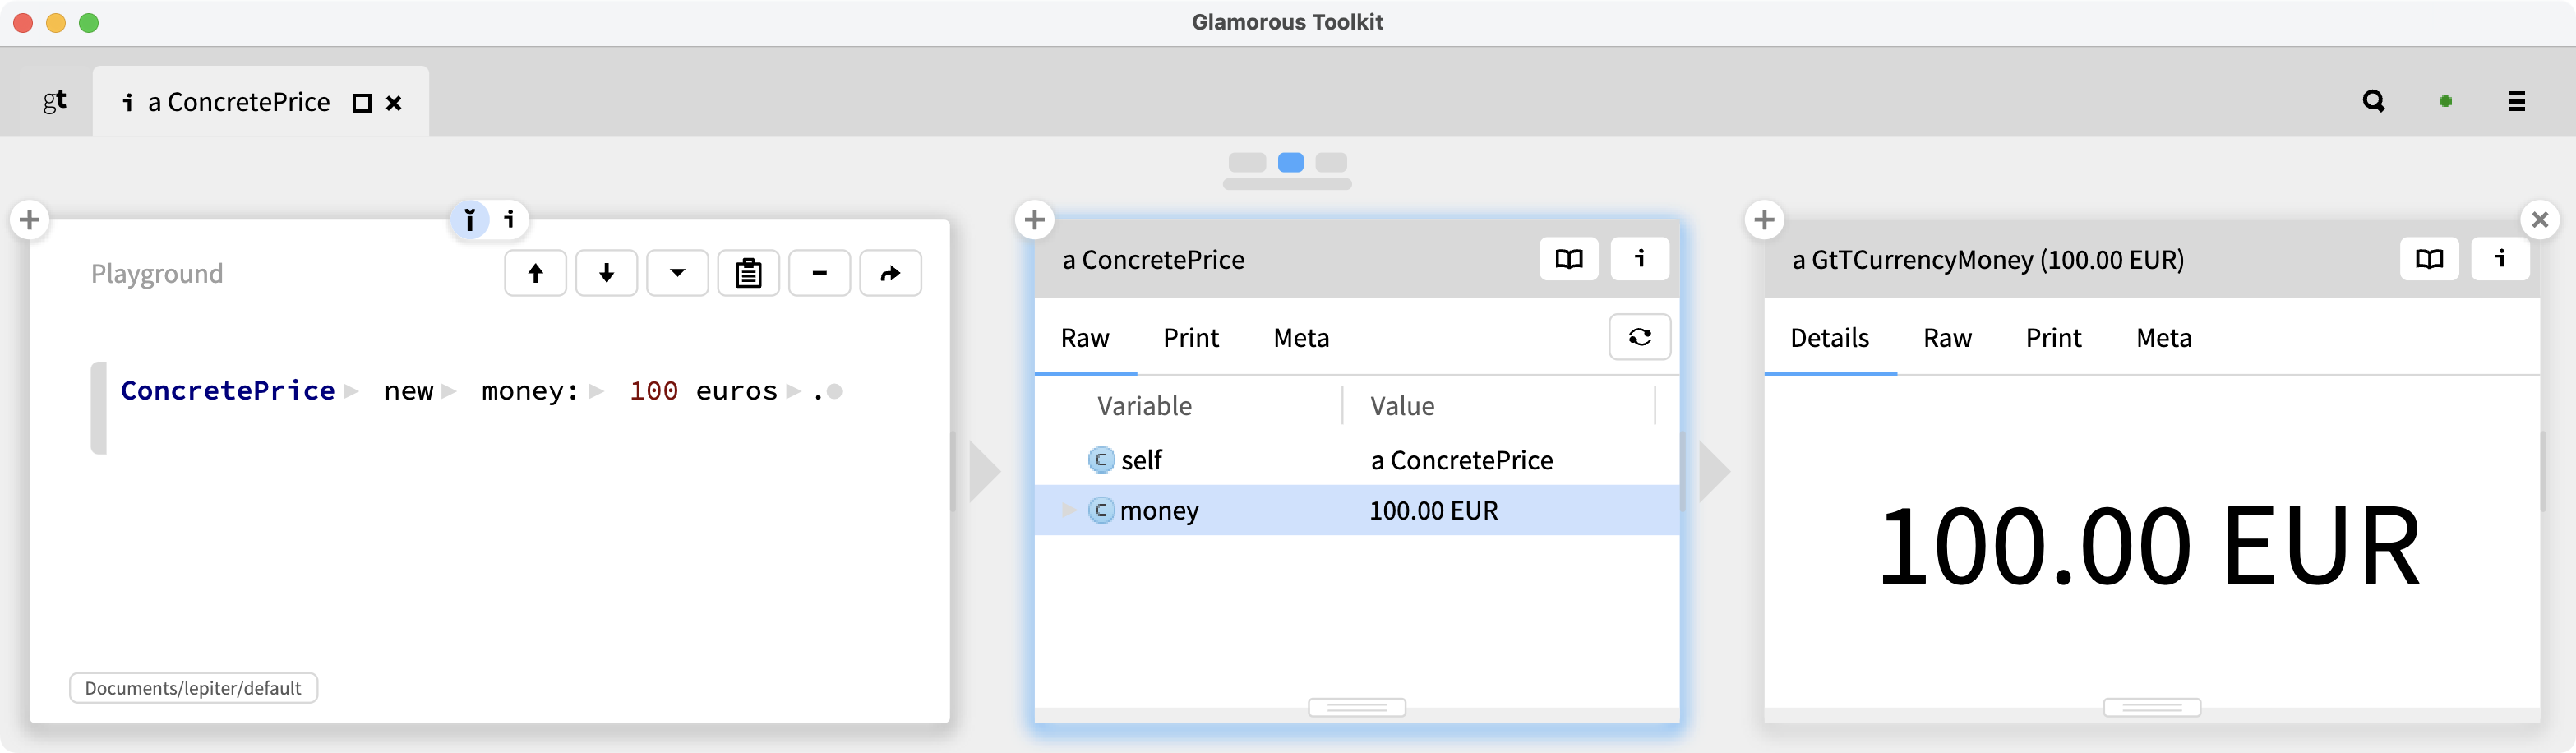
\includegraphics[width=\columnwidth]{edd1-ConcretePrice100Euros}
  \label{fig:exampleCreationA}
  }\qquad
\subfigure[xxx]{
  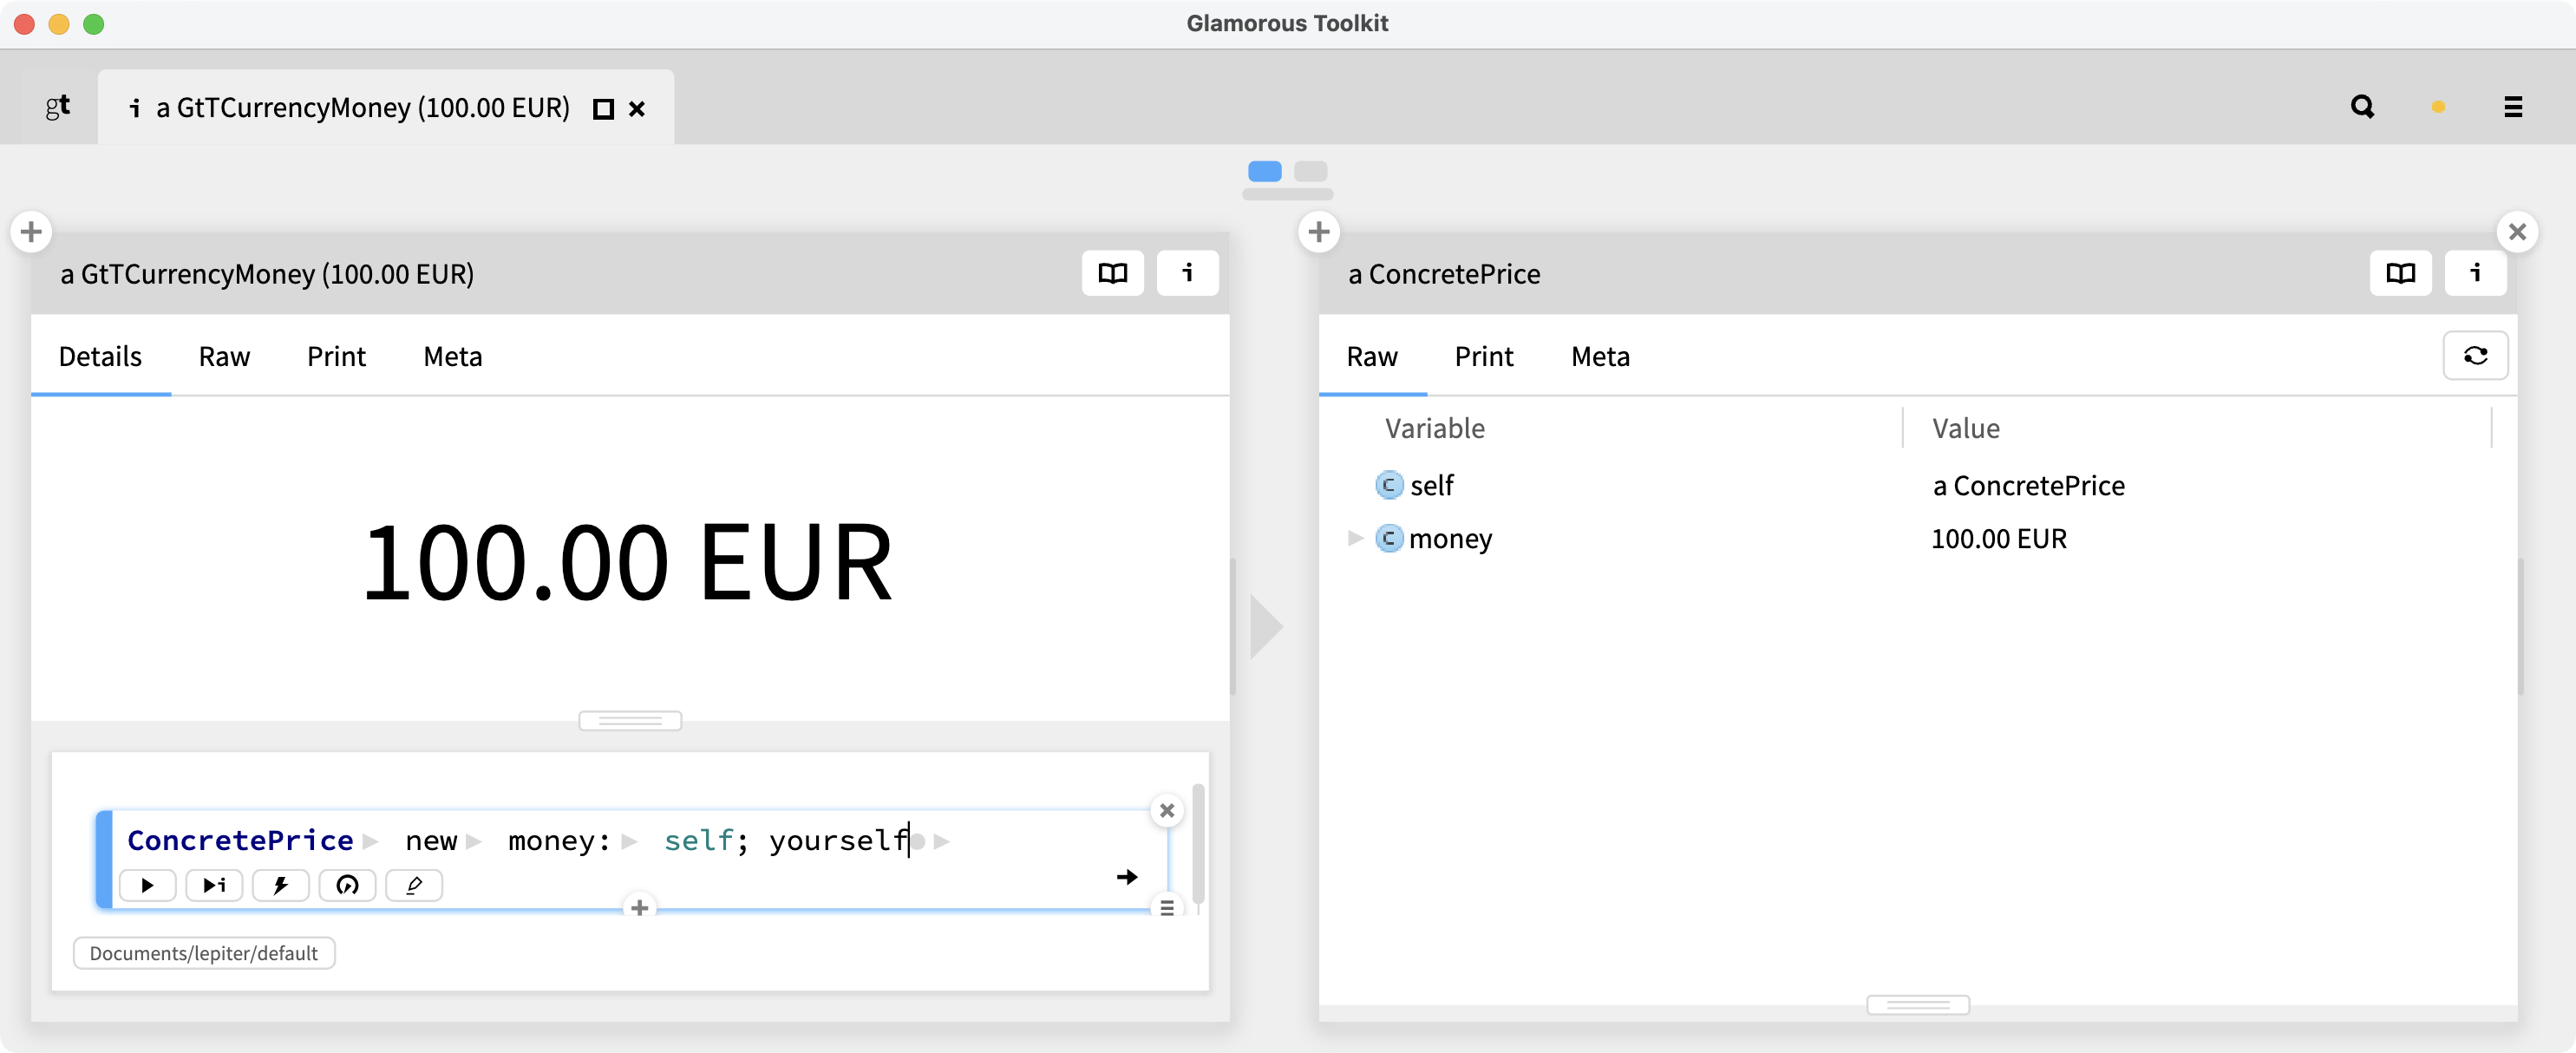
\includegraphics[width=\columnwidth]{edd2-PrototypingAsPrice}
  \label{fig:exampleCreationB}
  }\qquad
\subfigure[xxx]{
  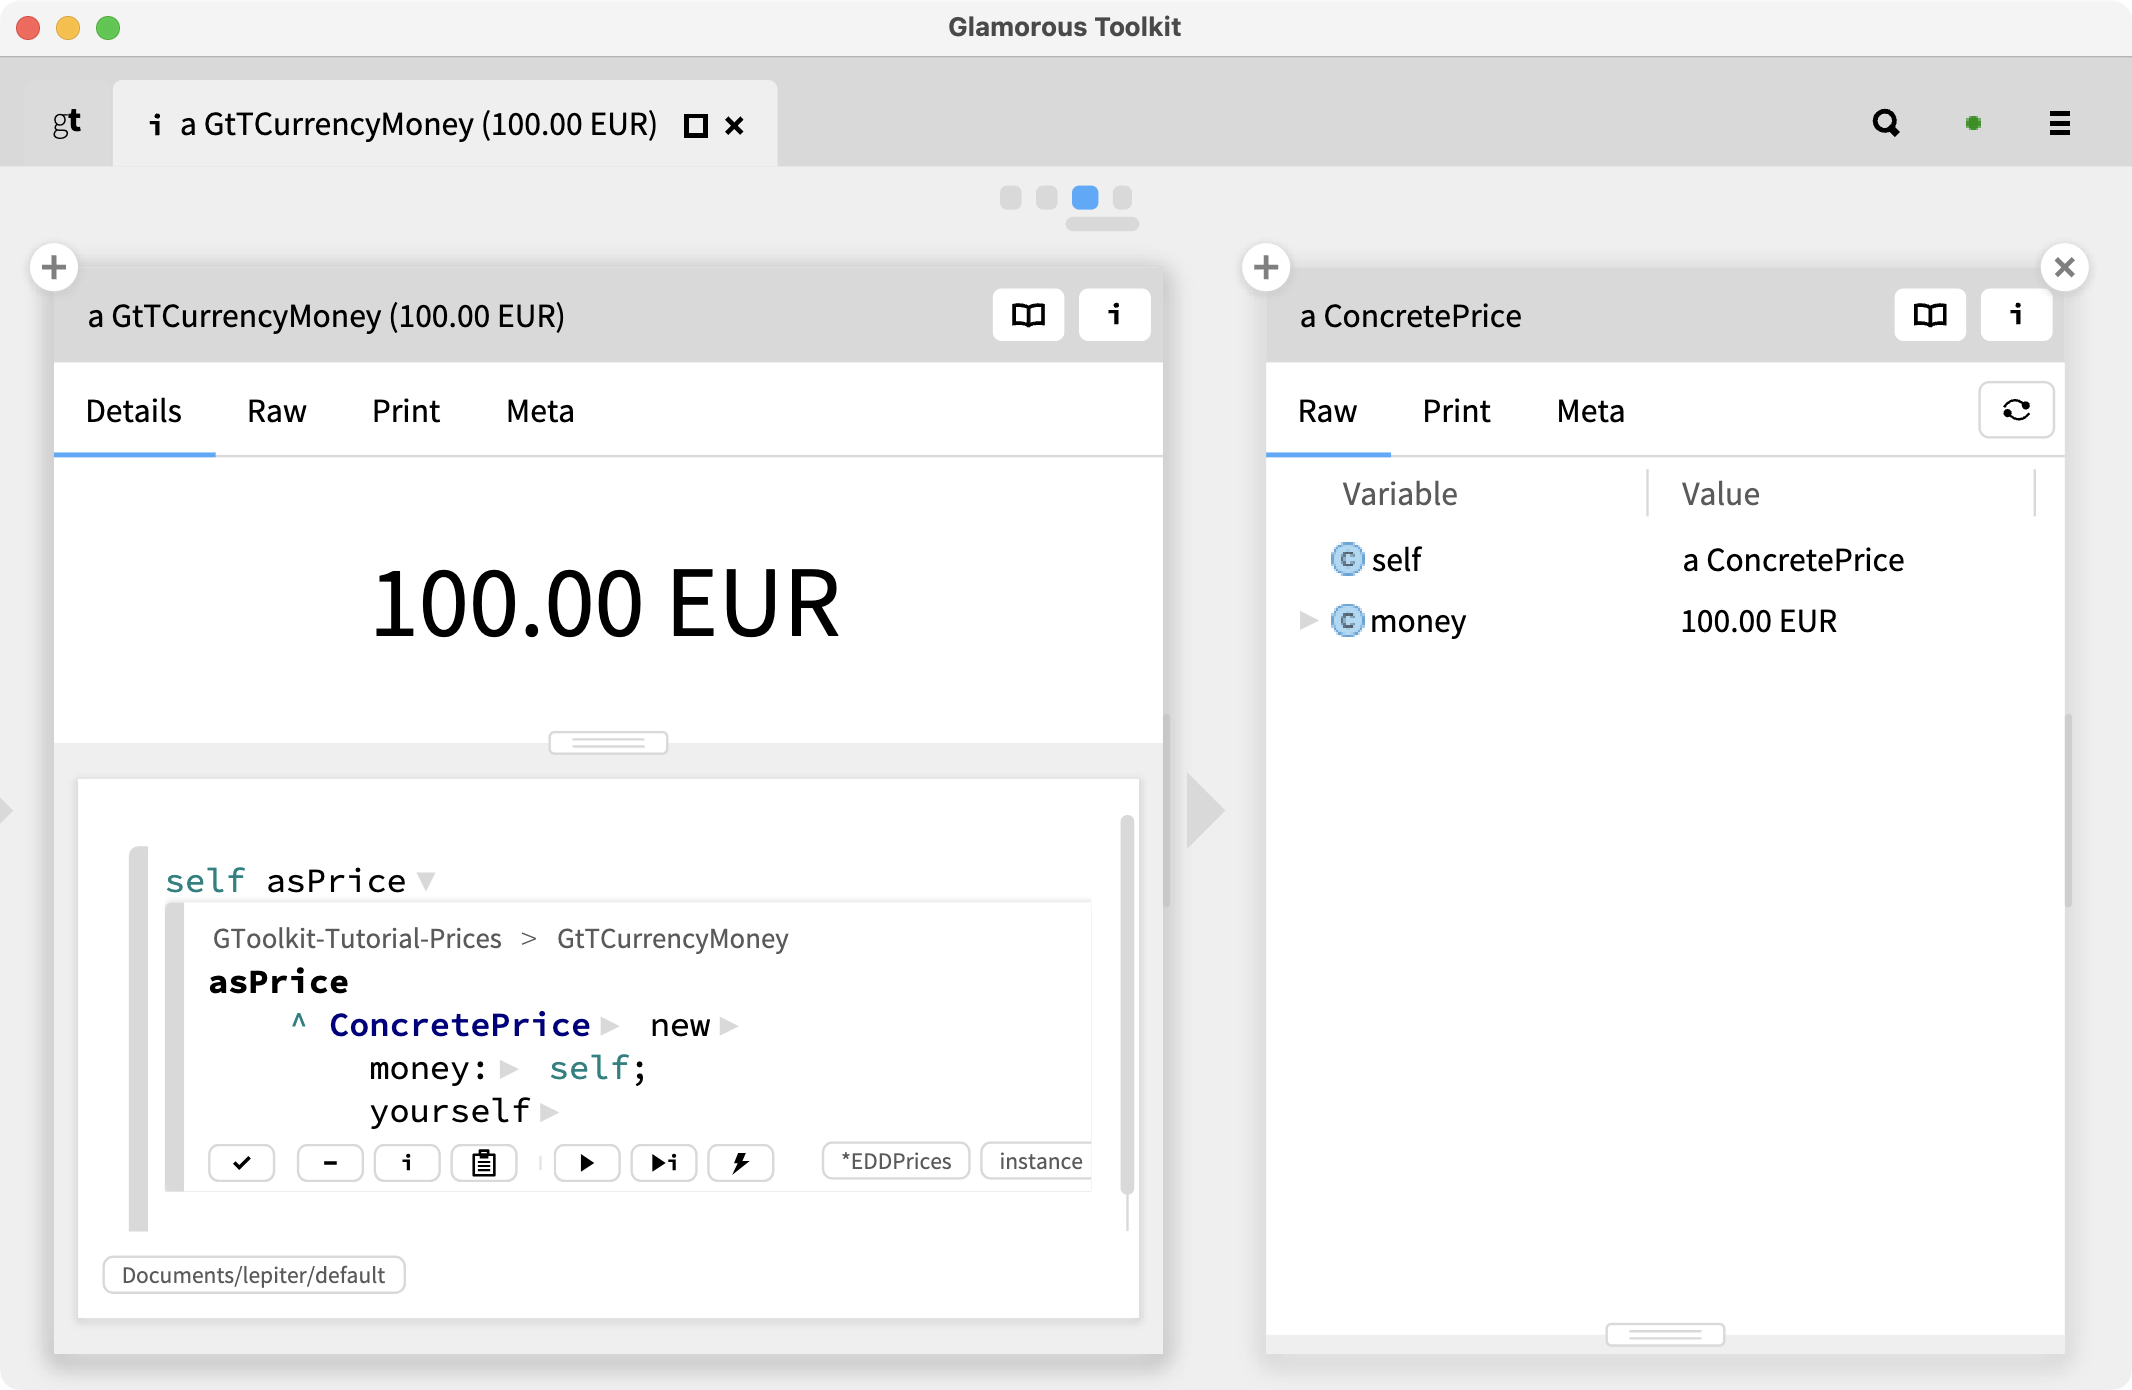
\includegraphics[width=\columnwidth]{edd3-ExtractAsPrice}
  \label{fig:exampleCreationC}
  }\qquad
\subfigure[xxx]{
  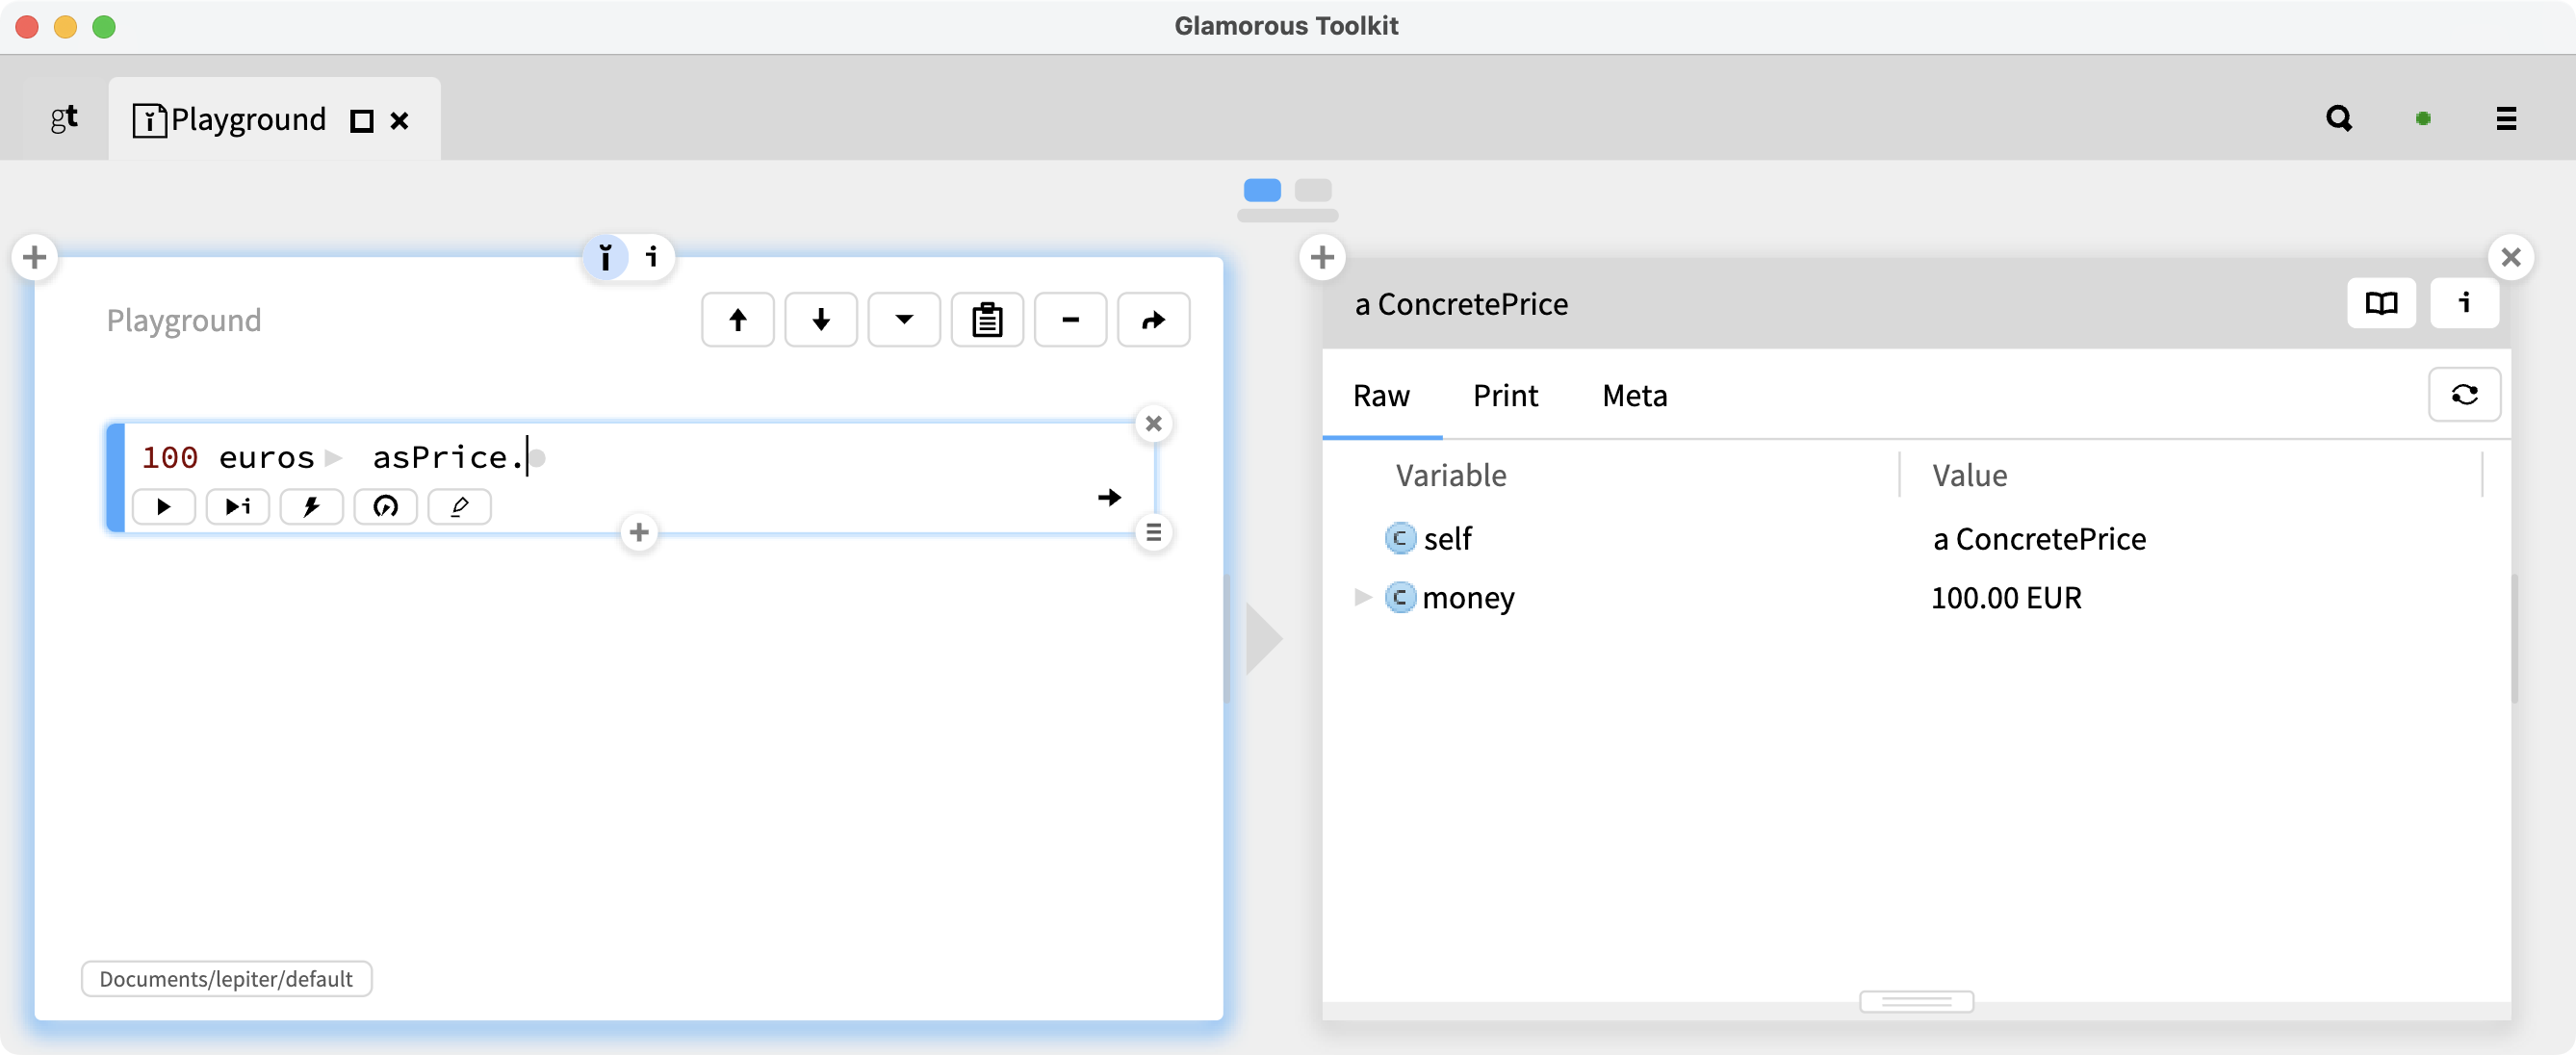
\includegraphics[width=\columnwidth]{edd4-MoneyAsPrice}
  \label{fig:exampleCreationC}
  }\qquad
  \caption{Building an example.}
  \label{fig:exampleCreation}
\end{figure}

Let's see how this can work with a small, running example.
Suppose we already have a library of classes implementing amounts of \st{Money} in various currencies.
Now we would like to implement \emph{prices} for goods, where a \st{Price} may be a concrete, fixed price, or a \emph{discounted} price, where the discount may be a fixed value or a percentage.

\here

\todo{Introduce GT}

Glamorous Toolkit (GT)\footnote{\url{https://gtoolkit.com}} ...

In \autoref{fig:exampleCreation} ...


In \autoref{fig:exampleExtraction} ...


\todo{Step through an EDD scenario as we did in the EDD blog.
Use the Prices use case?}
% https://lepiter.io/feenk/example-driven-development-ekmic0u0o8swpblzkcdzy608s/

\begin{figure}[ht]
\centering
\subfigure[xxx]{
  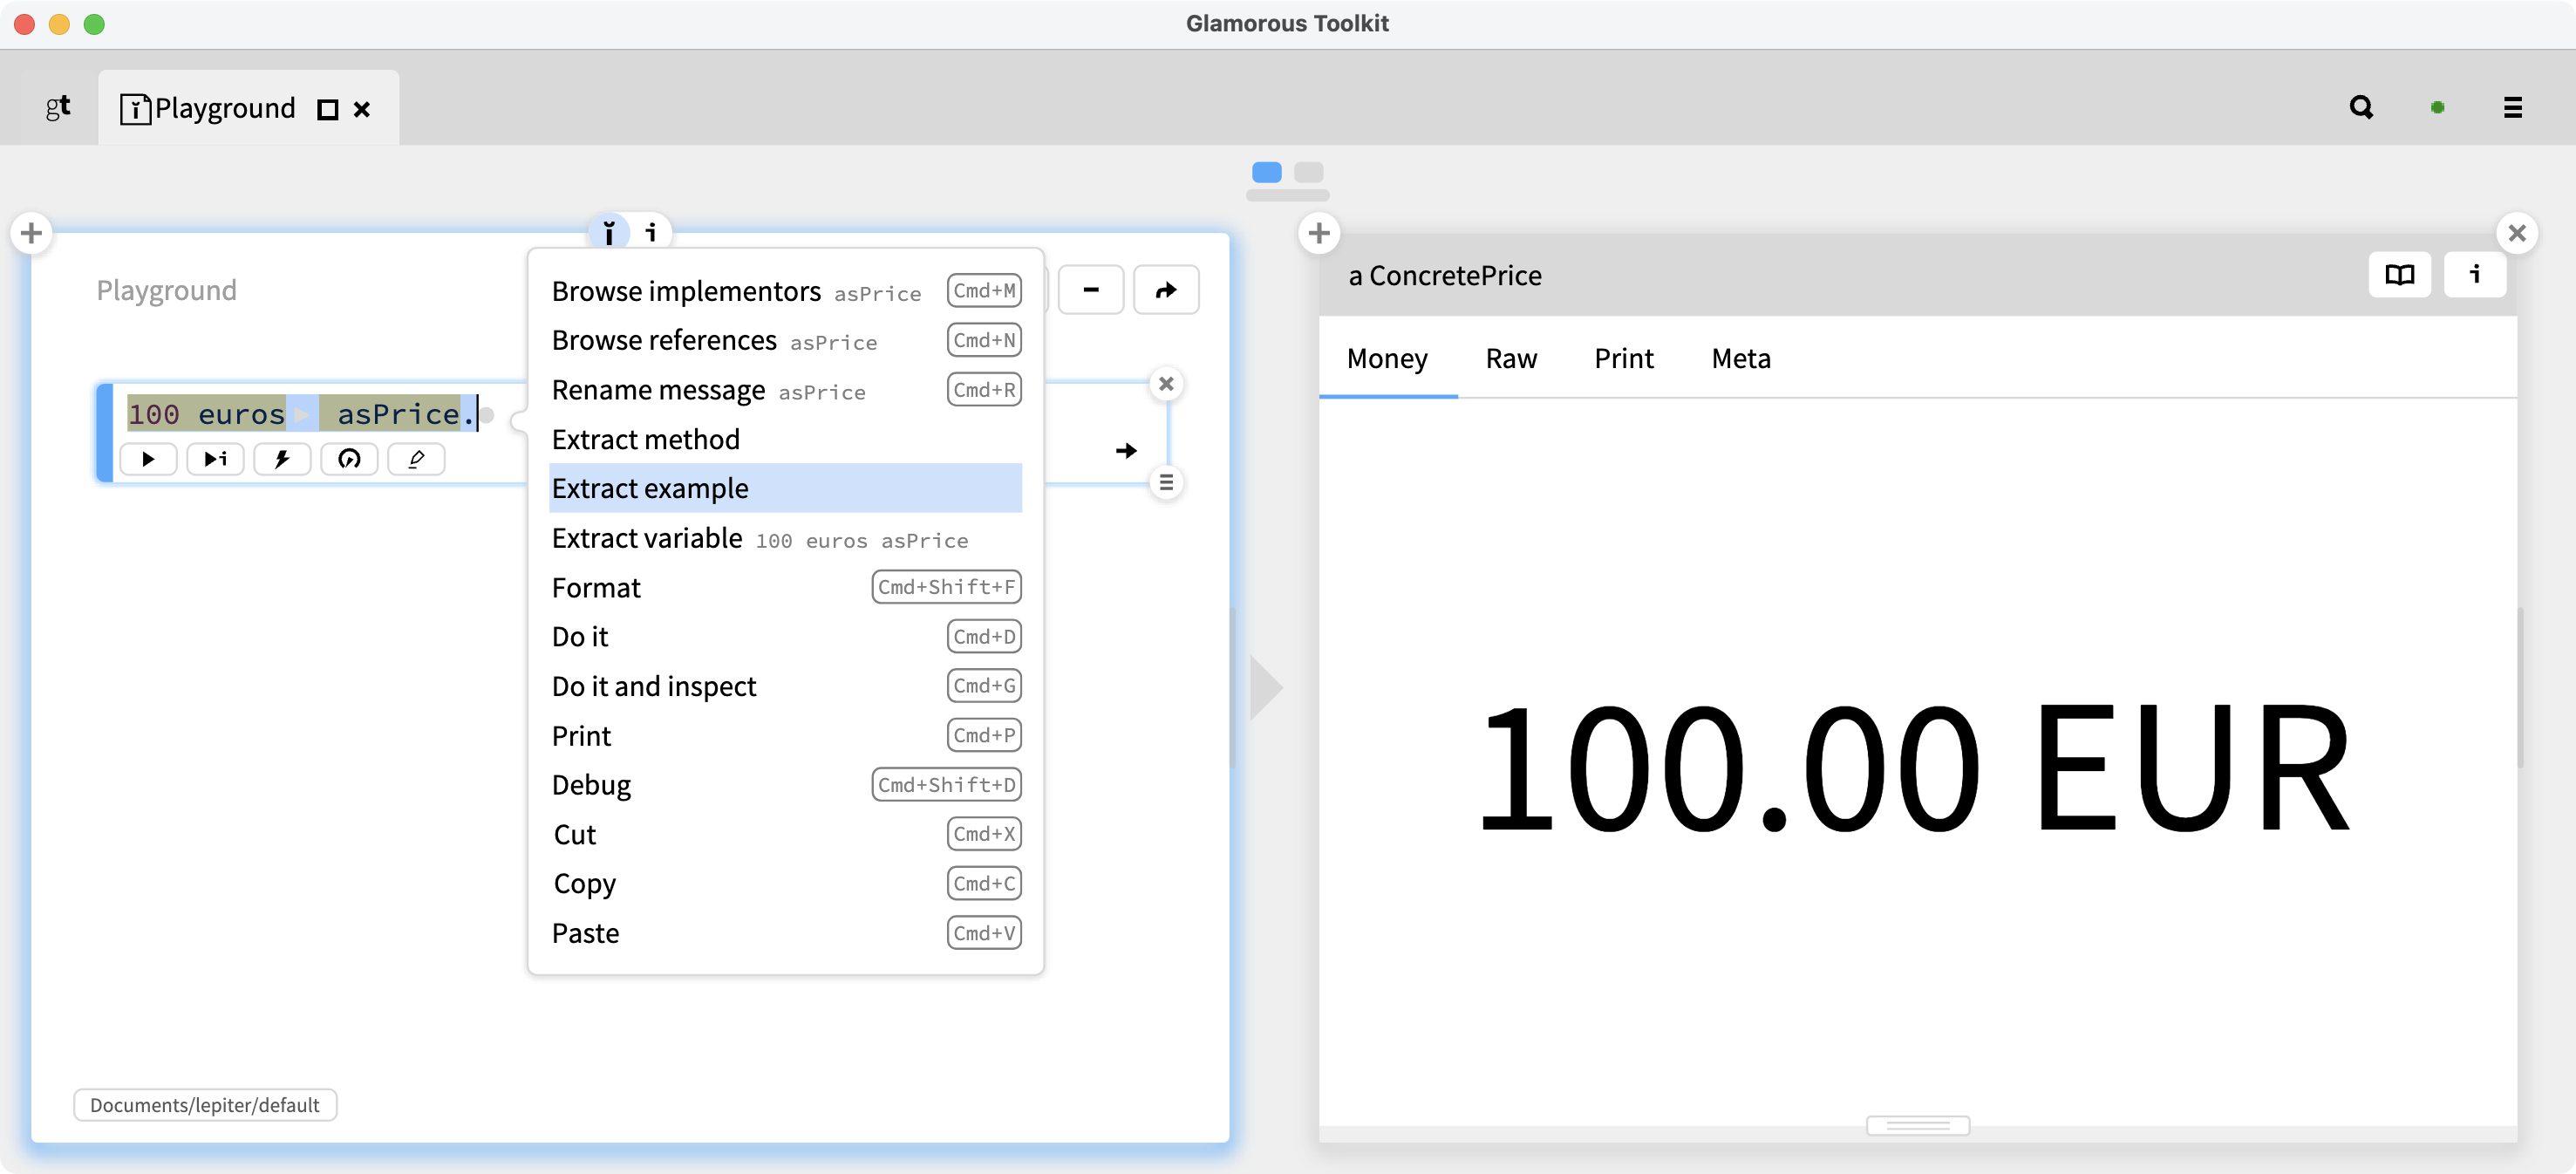
\includegraphics[width=\columnwidth]{edd5-ExtractingExample}
  }\qquad
\subfigure[xxx]{
  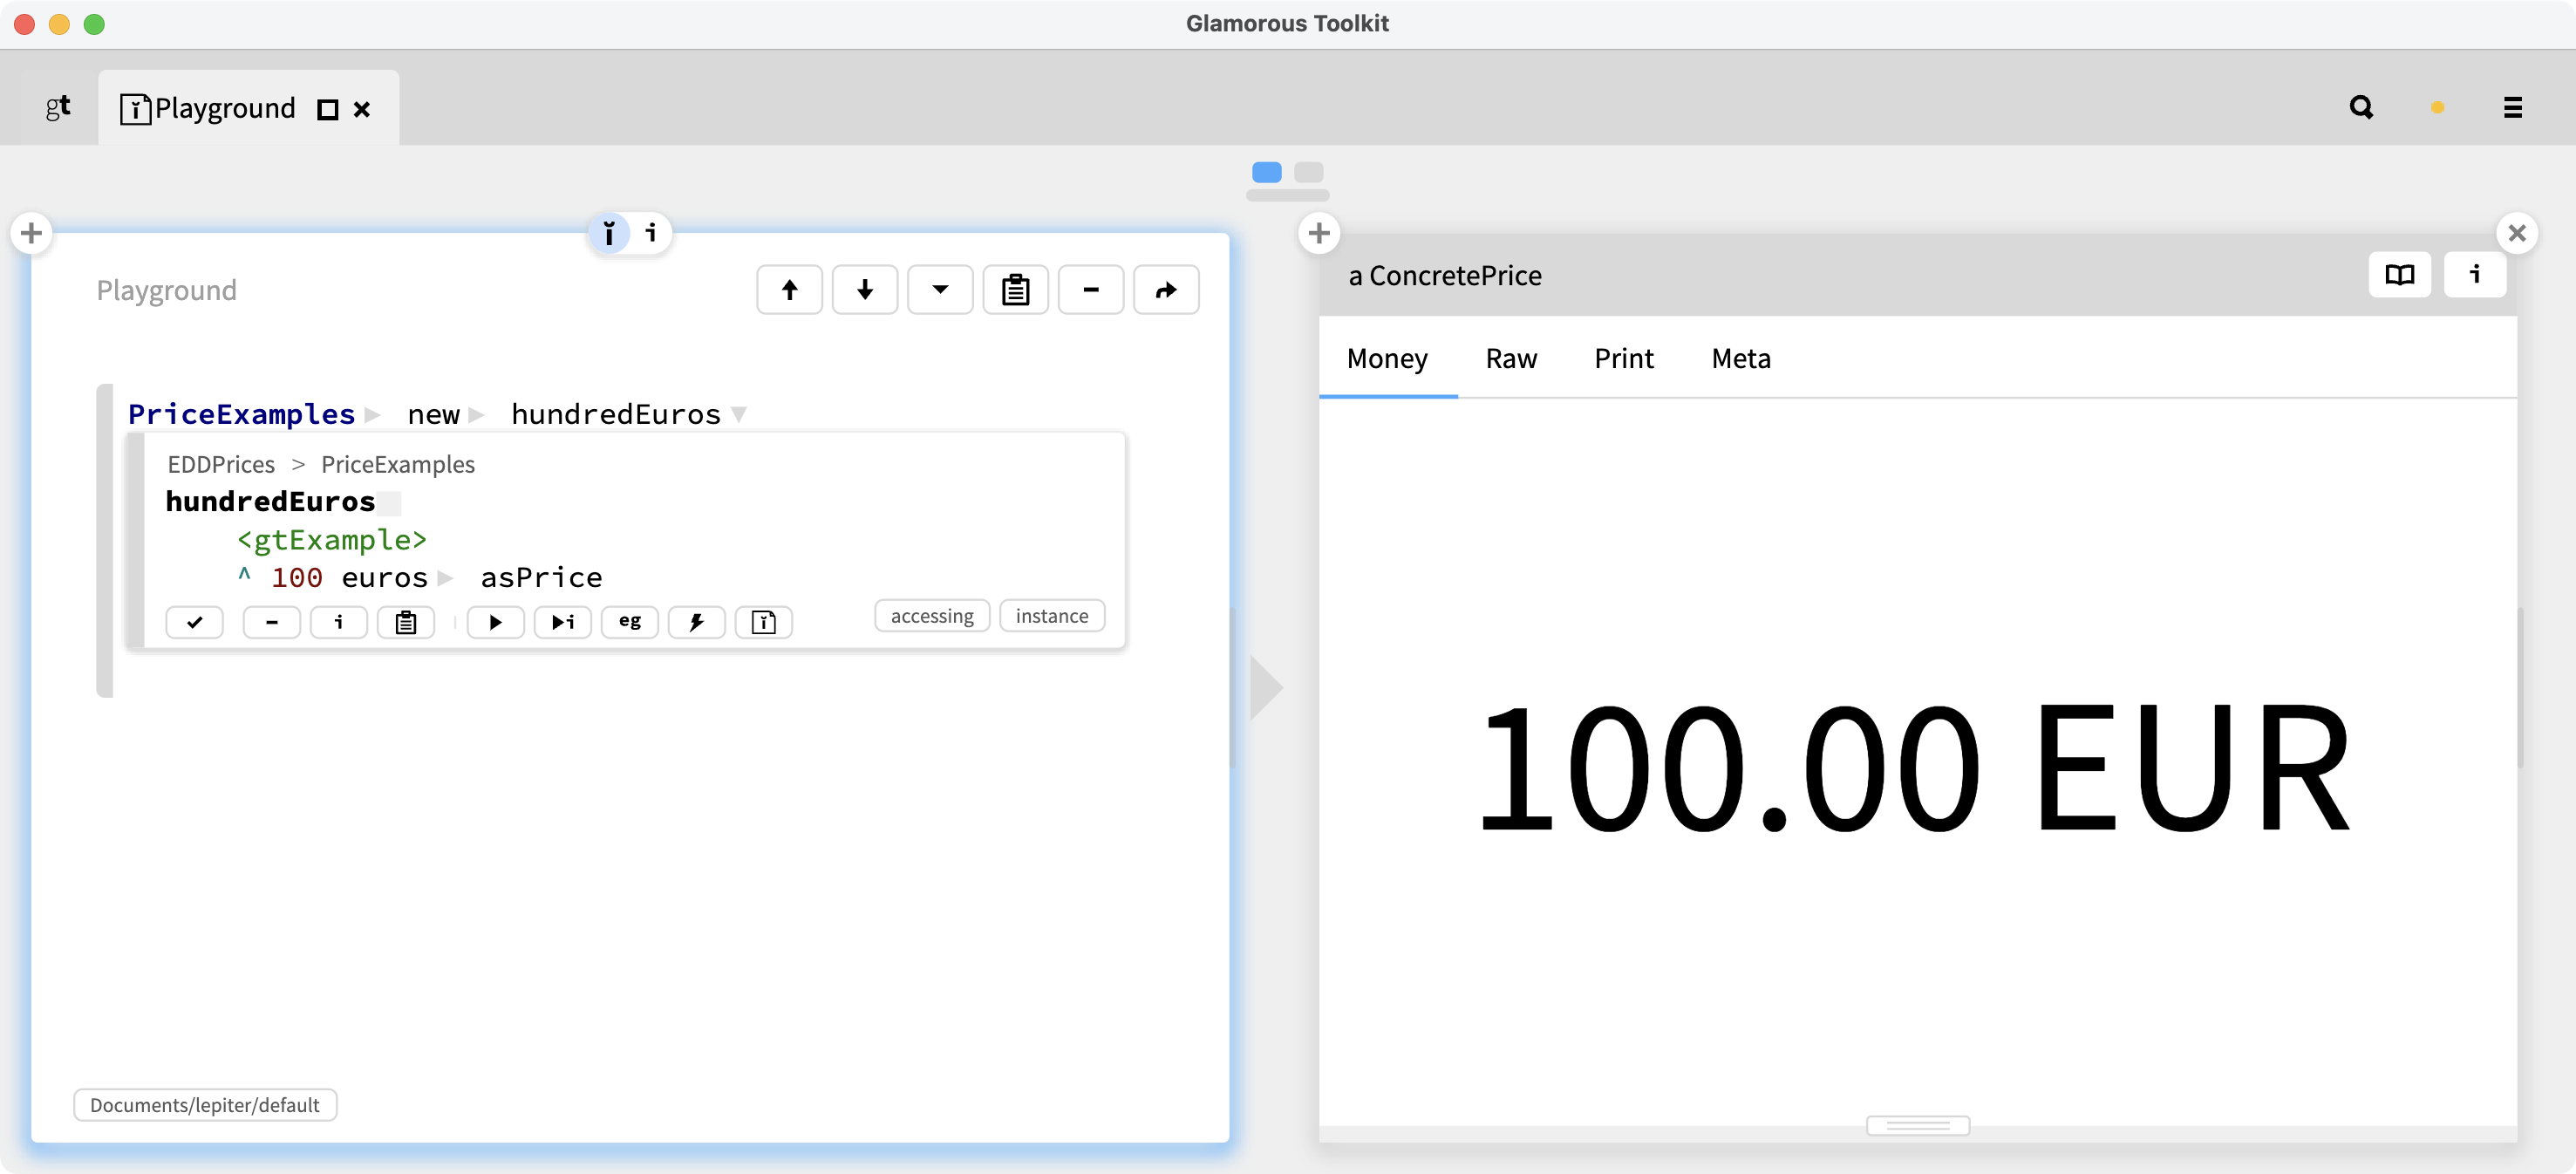
\includegraphics[width=\columnwidth]{edd6-PriceExample}
  }\qquad
\subfigure[xxx]{
  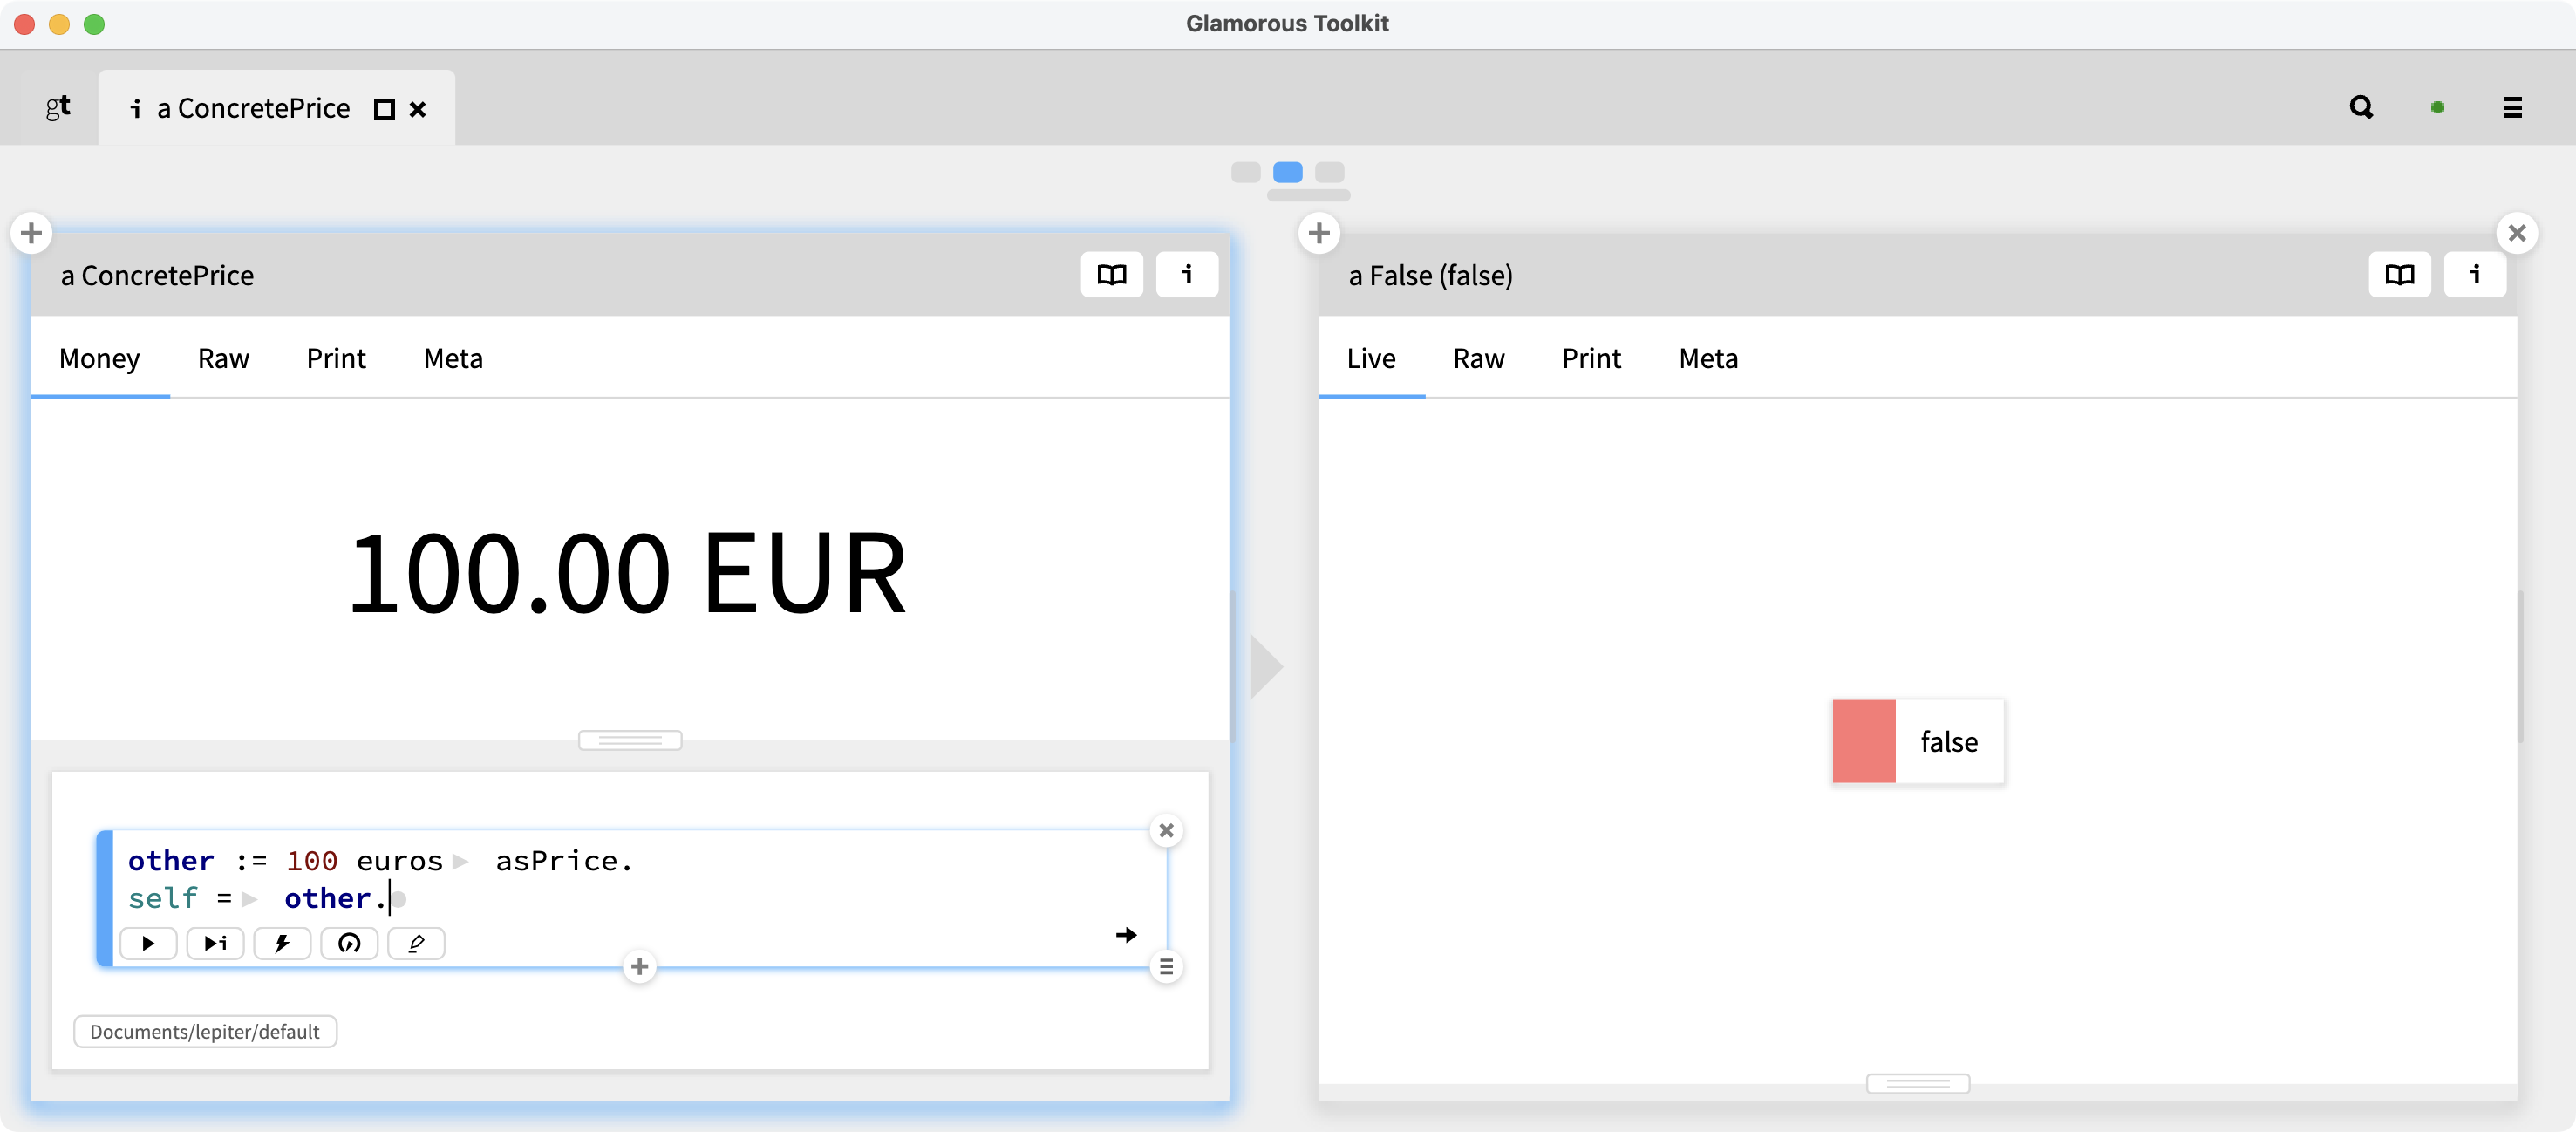
\includegraphics[width=\columnwidth]{edd7-FailedTest}
  }\qquad
%\subfigure[xxx]{
%  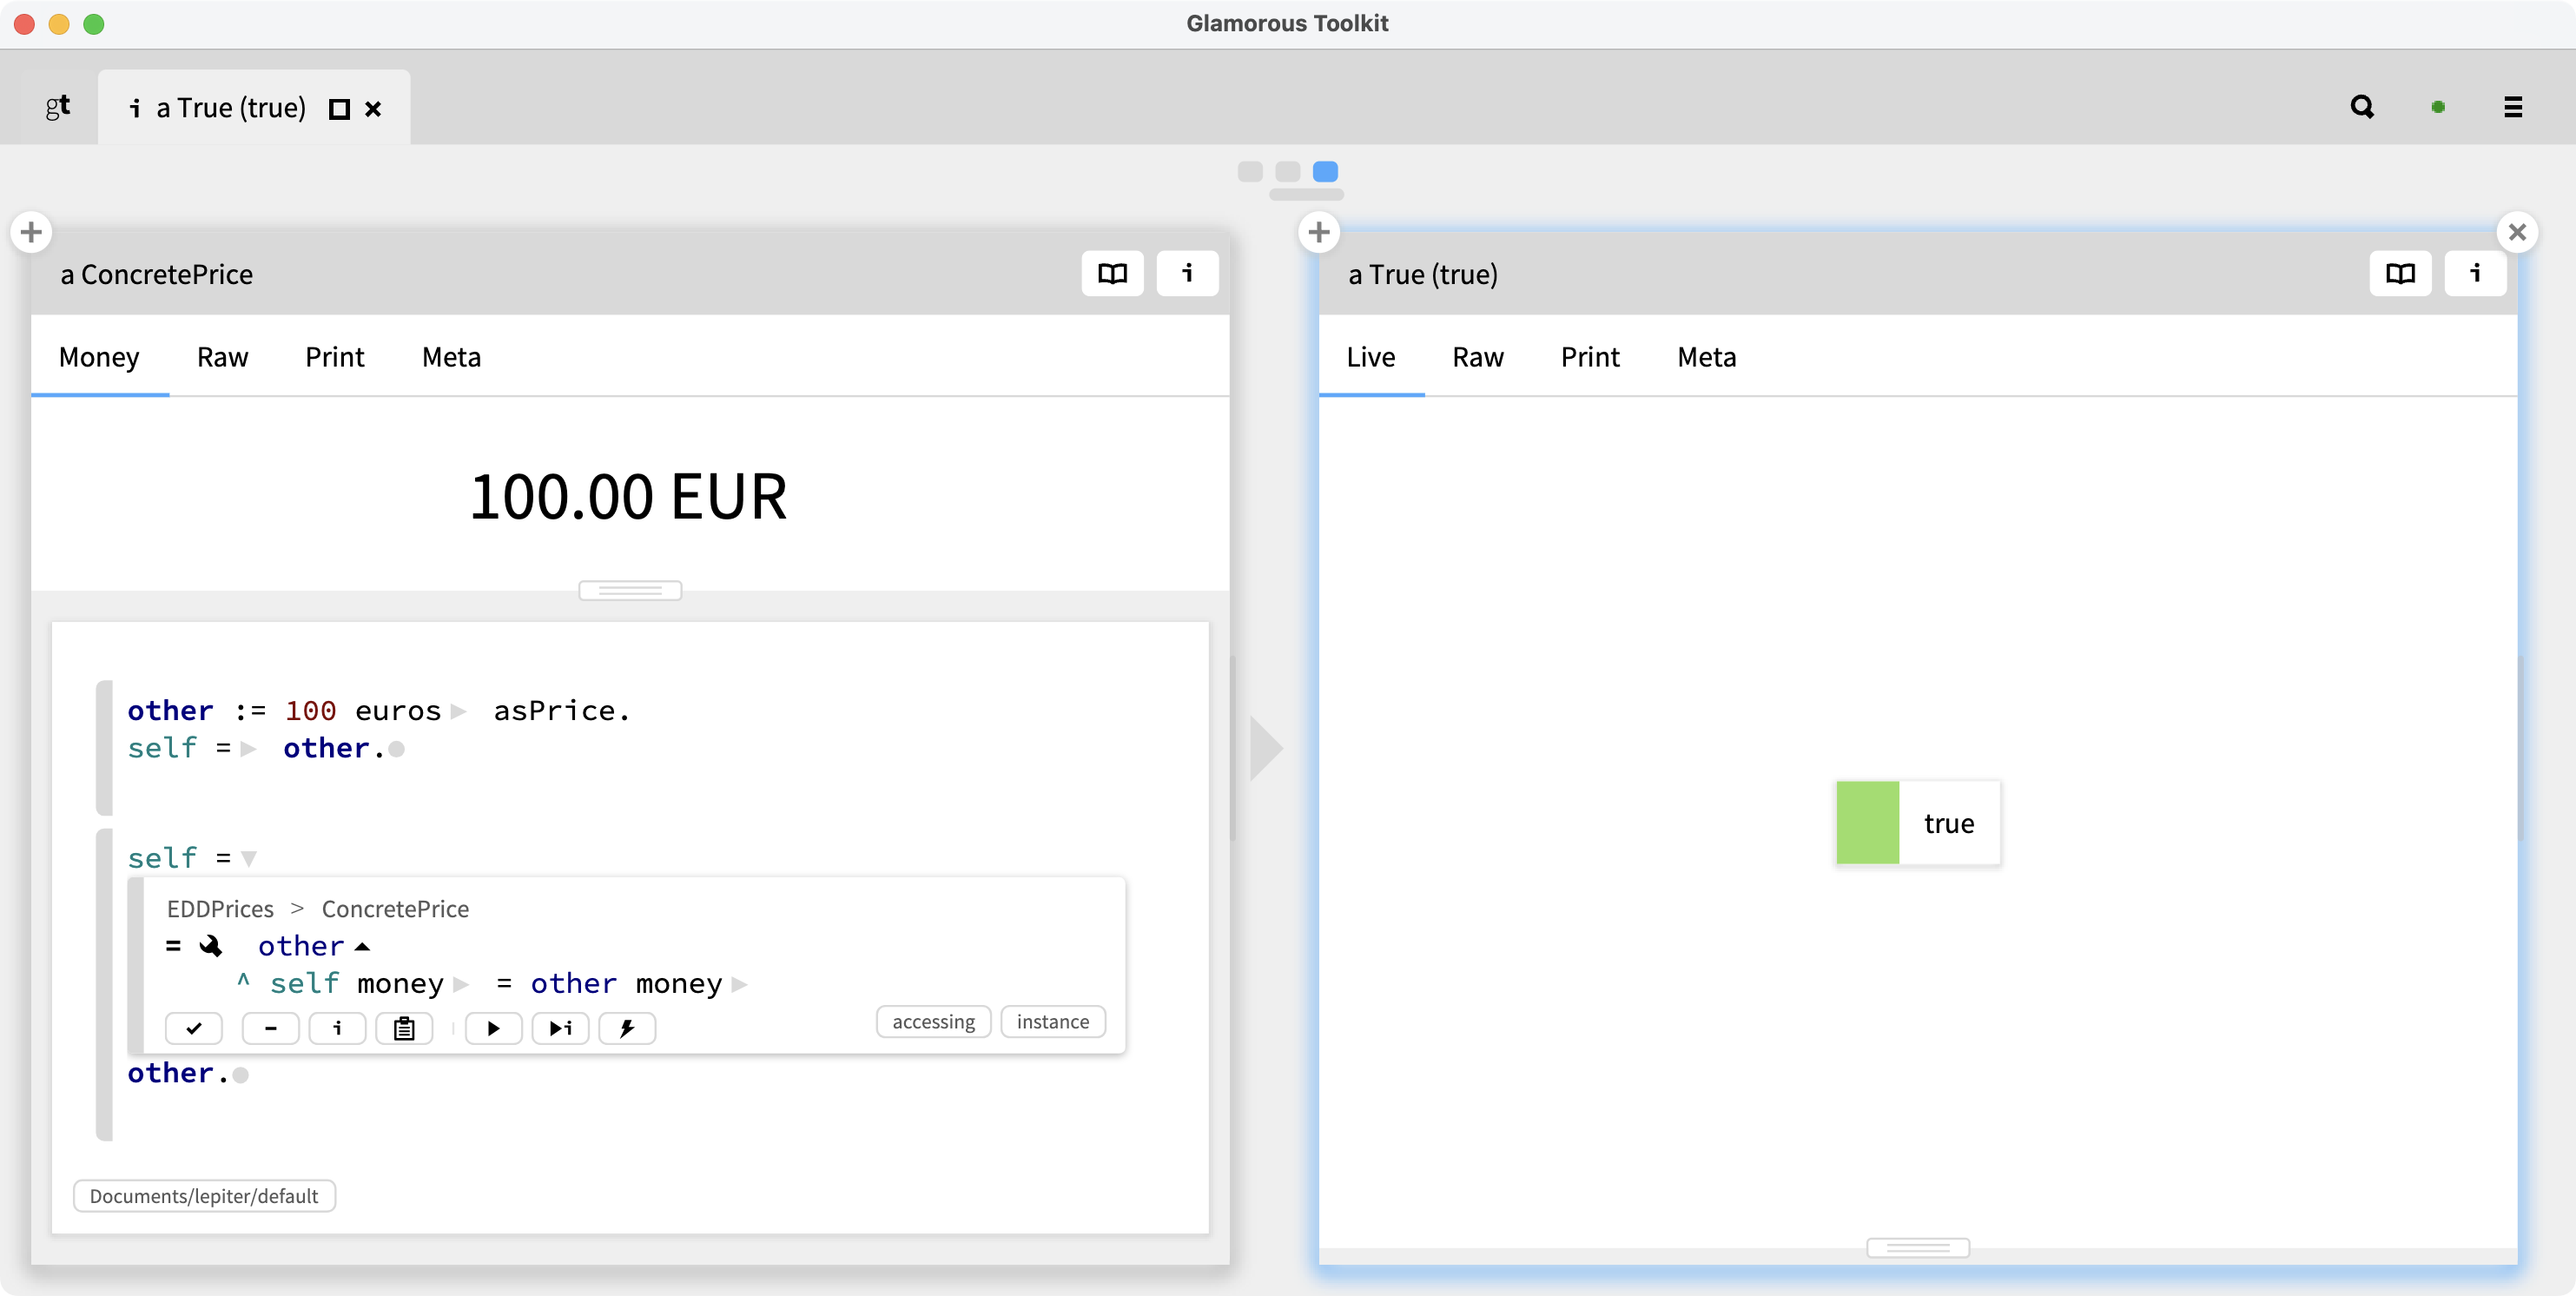
\includegraphics[width=\columnwidth]{edd8-ImplementingEquals}
%  }\qquad
\subfigure[xxx]{
  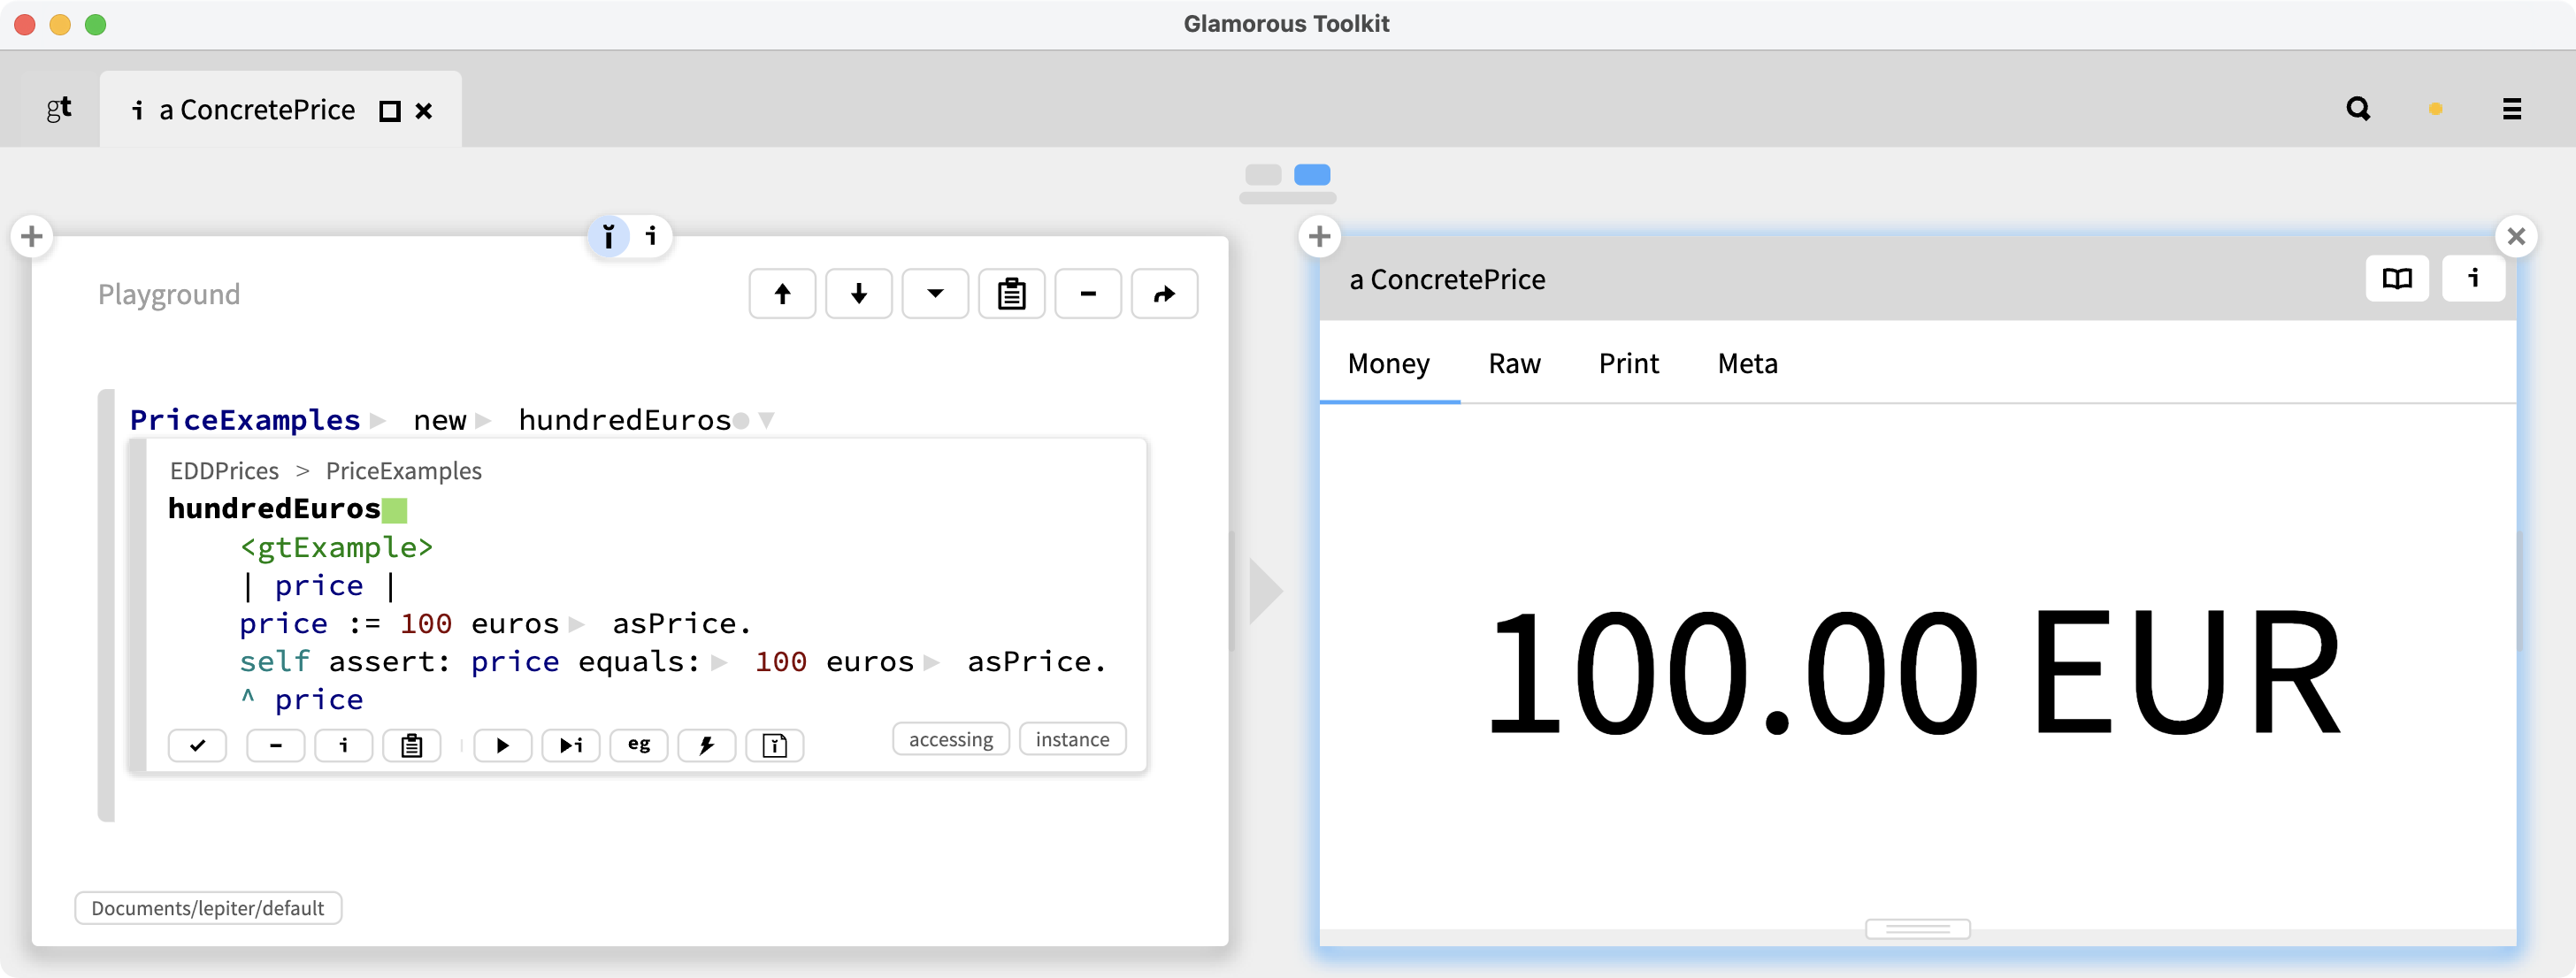
\includegraphics[width=\columnwidth]{edd9ExampleWithAssertions}
  }\qquad
  \caption{Extracting an example method.}
  \label{fig:exampleExtraction}
\end{figure}


% ============================================================
\section{Moldable Examples}\label{sec:moldable}

\emph{Moldable development} is an approach to constructing \emph{explainable software systems} by augmenting the objects of the software system with dozens of tiny analysis tools that can answer questions about the system.
It can be understood as a refinement of EDD in which objects (examples) are enhanced with custom tools during the development process.

Moldable development is made possible with the help of \emph{moldable tools}~\cite{Chis17a}, such as code browsers, debuggers, and object inspectors, that can adapt themselves to the run-time context of an application to enable these analysis tools.
% Chis17a Moldable Tools for Object-oriented Development
For example, consider the screenshot of the Ludo\footnote{\url{https://en.m.wikipedia.org/wiki/Ludo}} in figure \autoref{fig:ludoViews}.
At the left we see in an object inspector a GUI \emph{Board} view of a running instance of the game that has terminated with player B winning.
In the middle we see a \emph{Moves} view of the same instance, showing us all the past moves leading to the concluding state of the game.
Finally, at the right we inspect a particular move, showing us how the game state was updated in move \#109.

\begin{figure}[h]
  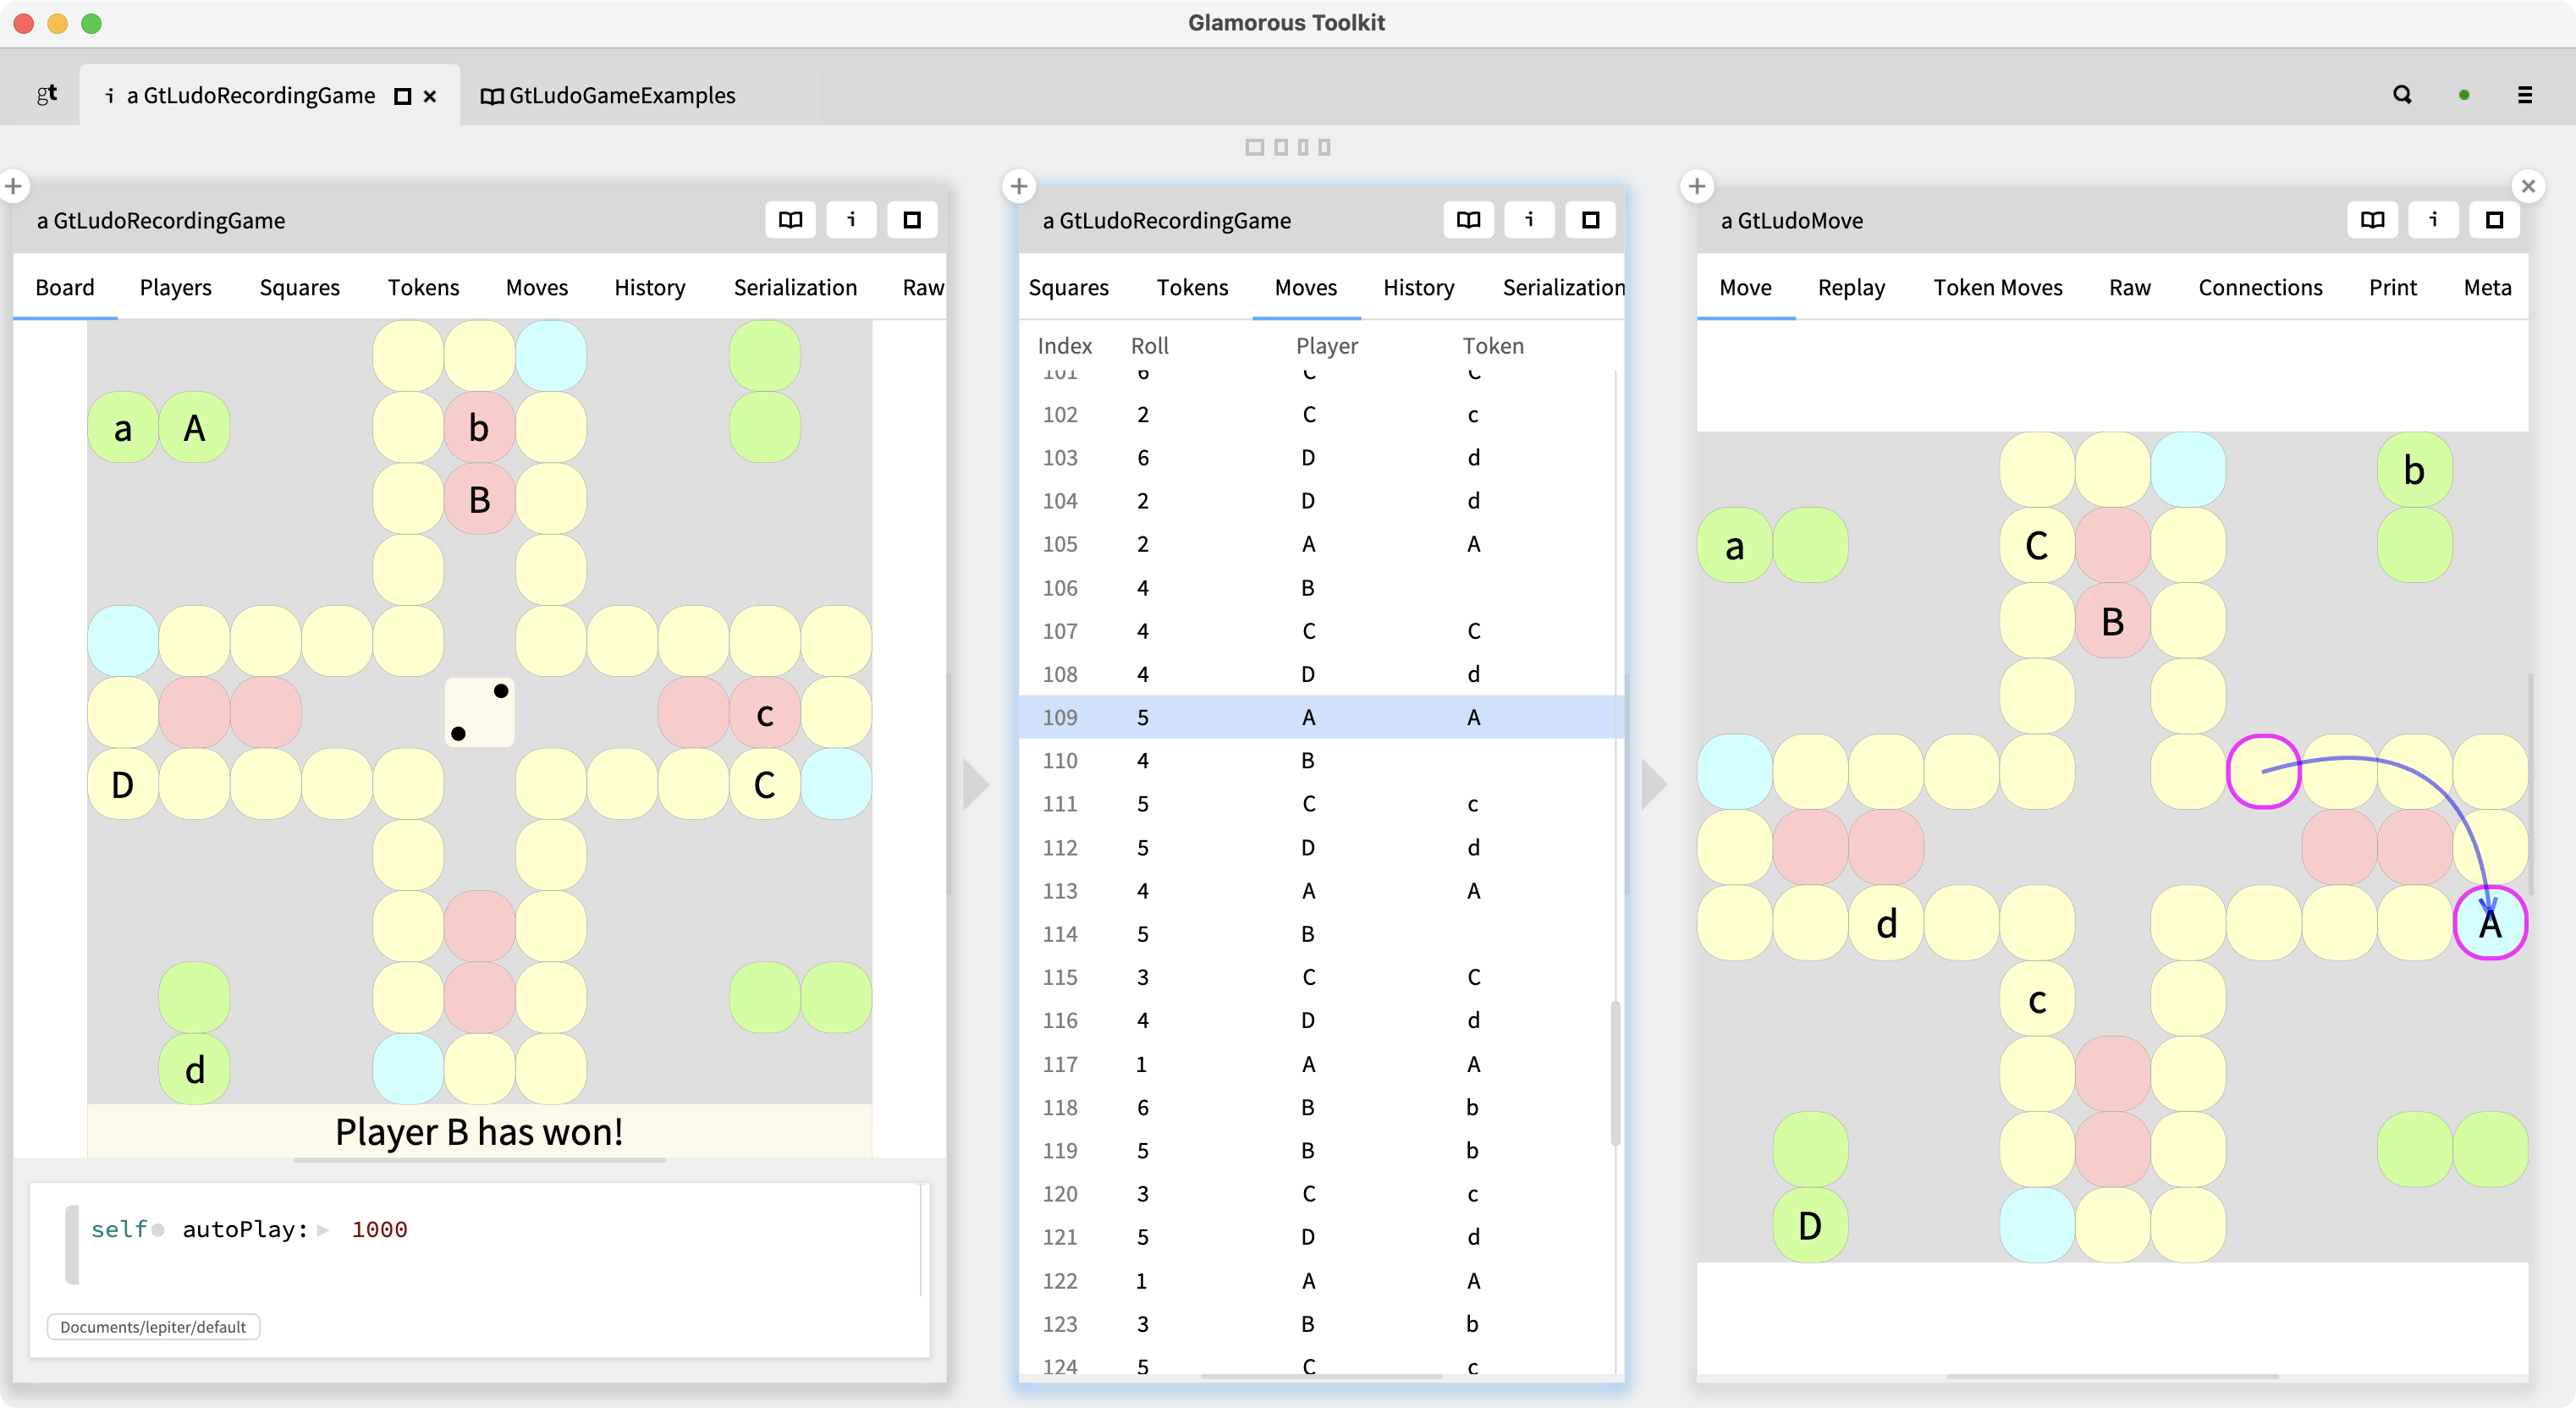
\includegraphics[width=\columnwidth]{customViews}
  \caption{Custom views of a Ludo game.}
  \label{fig:ludoViews}
\end{figure}

These views have each been created with a few lines of code, in the first and last cases leveraging the existing GUI view of the Ludo game.
The object inspector recognizes that the Ludo game object is an instance of the \lst{GtLudoRecordingGame} class, 
which has been extended with several custom views defined as annotated methods of that class.
Similarly the move object is an instance of the \st{GtLudoMove} class, which has been extended with other views specific to moves.

Two other common types of custom tools are \emph{custom actions} (\eg buttons), which perform a task and possible spawn another tool such as an inspector, a code editor or an external web browser, and \emph{custom searches}, which query the running object model and spawn a tool such as an object inspector on the result.

Examples are both the input and output of moldable development.
Typically we start with a ``raw'', unenhanced example, such as we see in \autoref{fig:exampleCreation}: the \st{aConcretePrice} inspector views all show just a basic view of the instance state of the example.
As we elaborate the examples in the EDD process, we mold them with custom tools that validate the requirements expressed by the examples.
The output of the process is then a molded example that not only checks assertions about its expected behavior, but also exposes that behavior through custom tools.

Let's see how this works.
\todo{Go back to the Price examples from the last section, and see how custom tools enhance the examples}

\autoref{fig:ConcretePrice}
\autoref{fig:DiscountedPrice}


\begin{figure}[h]
  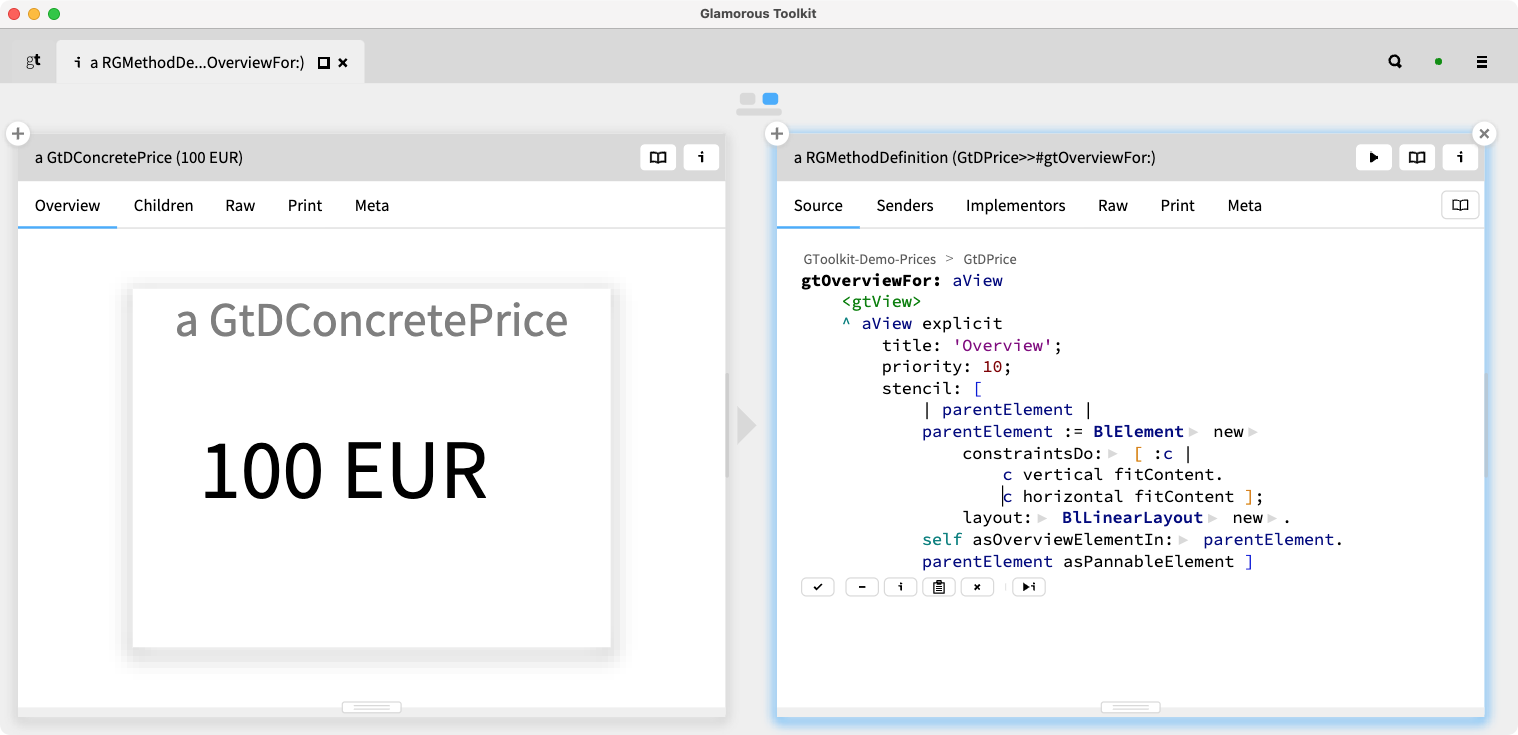
\includegraphics[width=\columnwidth]{md1-ConcretePrice}
  \caption{xxx.}
  \label{fig:ConcretePrice}
\end{figure}




\begin{figure}[h]
  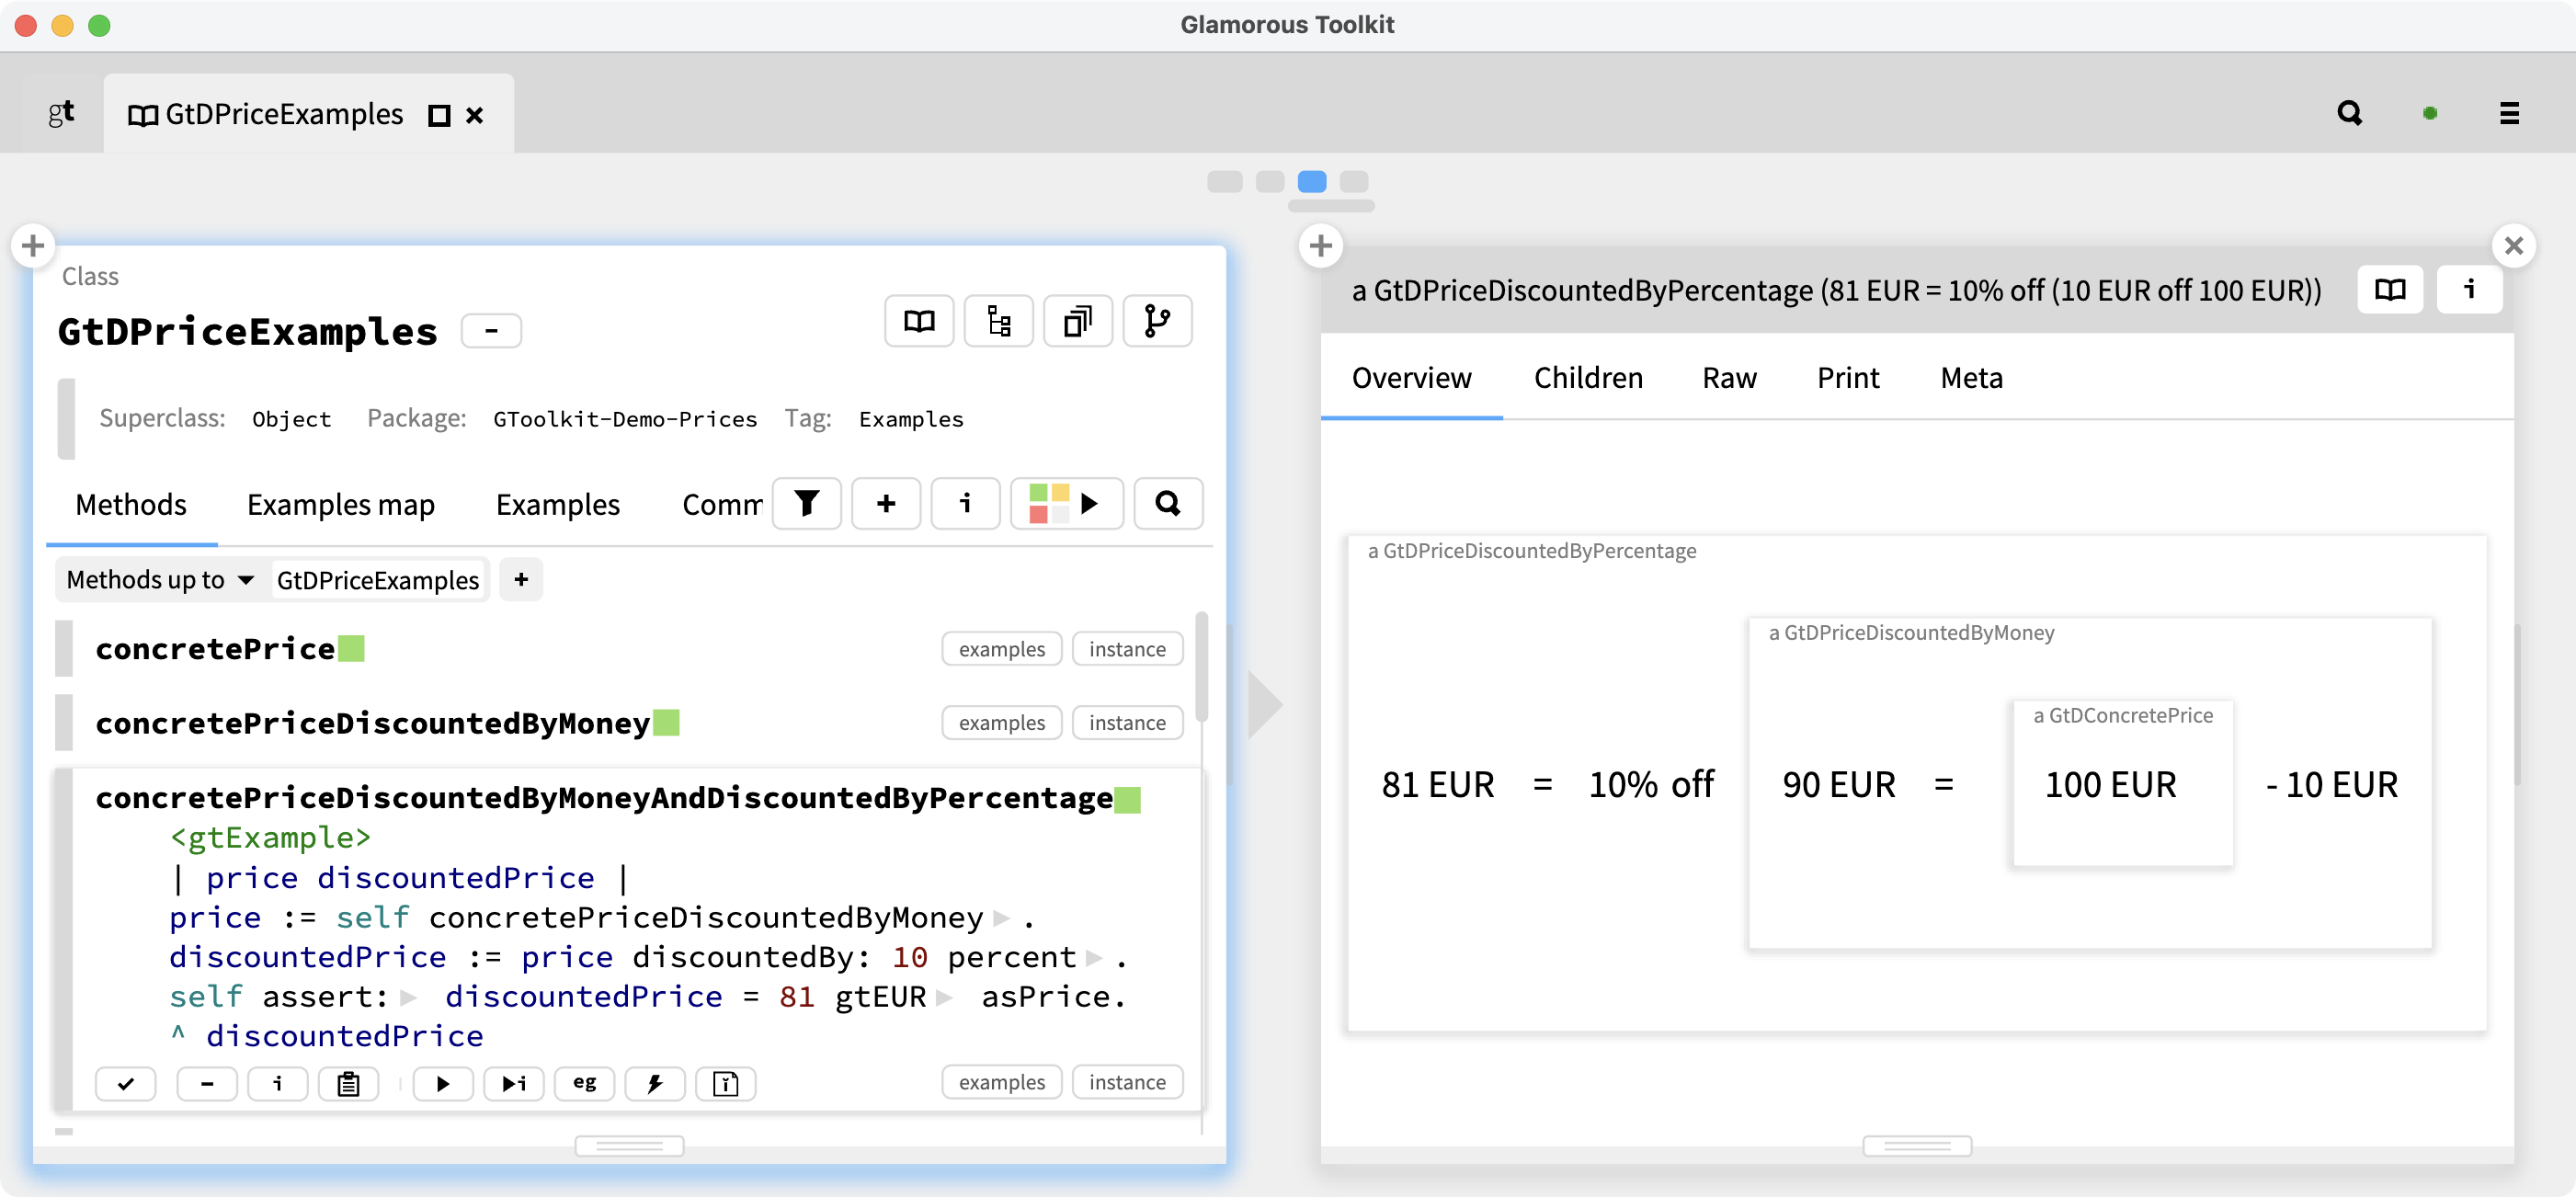
\includegraphics[width=\columnwidth]{md2-DiscountedPrice}
  \caption{xxx.}
  \label{fig:DiscountedPrice}
\end{figure}





% ============================================================
\section{Explainable Systems using Examples}\label{sec:explainable}

\todo{Add something about creating narratives -- the custom views allow you to create both fixed narratives as notebook pages, and dynamic narratives by navigating to new views}

Perhaps the most compelling use of examples is within live documentation.
GT includes support for knowledge bases consisting of linked notebook pages that are composed various kinds of snippets: formatted test, images, code in various programming languages, and live examples.
An example snippet identified an example method to be evaluated, and a views to be rendered when the notebook page is loaded.

This simple feature enables the creation of various kinds of live documentation, such as live project diaries, interactive tutorials, and live API documentation.

Let's see a few examples from the GT book, the knowledge base that comes bundled with the GT download.

In \autoref{fig:Memory} we see pages of a tutorial explaining how to build a graphical user interface using examples of a ``Memory'' game.
\todo{explain the figure}


\begin{figure}[h]
  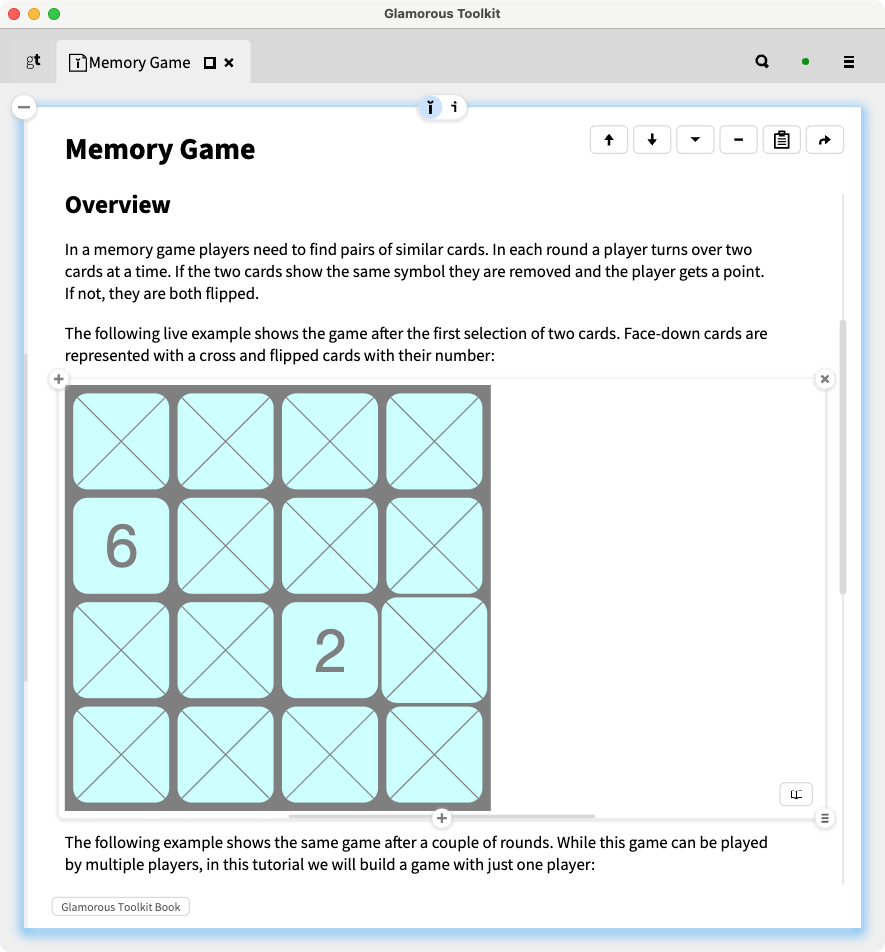
\includegraphics[width=\columnwidth]{book1-Memory}
  \caption{xxx.}
  \label{fig:Memory}
\end{figure}




\autoref{fig:SPL} explains how to implement a simple programming language using the PetitParser framework that comes bundled with GT.
\todo{explain the figure}



\begin{figure}[h]
  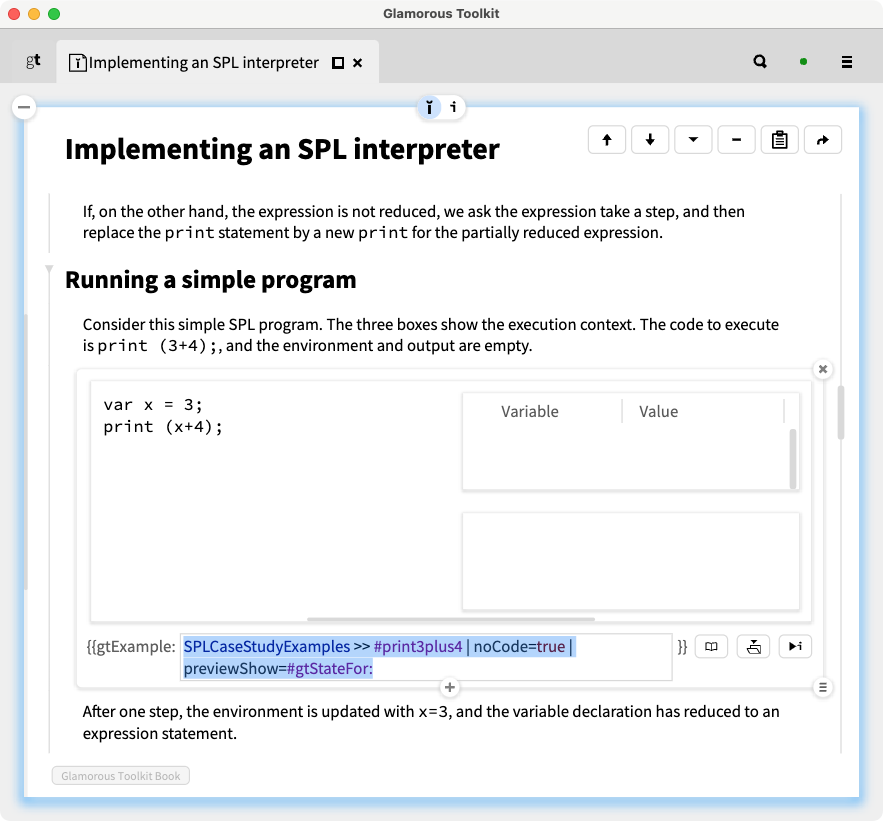
\includegraphics[width=\columnwidth]{book2-SPL}
  \caption{xxx.}
  \label{fig:SPL}
\end{figure}

\st{SPLCaseStudyExamples >> #print3plus4 | noCode=true | previewShow=#gtStateFor:}


Examples can also be used effectively to explain algorithms.
In \autoref{fig:Treemap} we see a notebook page that explains how a treemap layout algorithm works with the help of live examples.



\begin{figure}[h]
  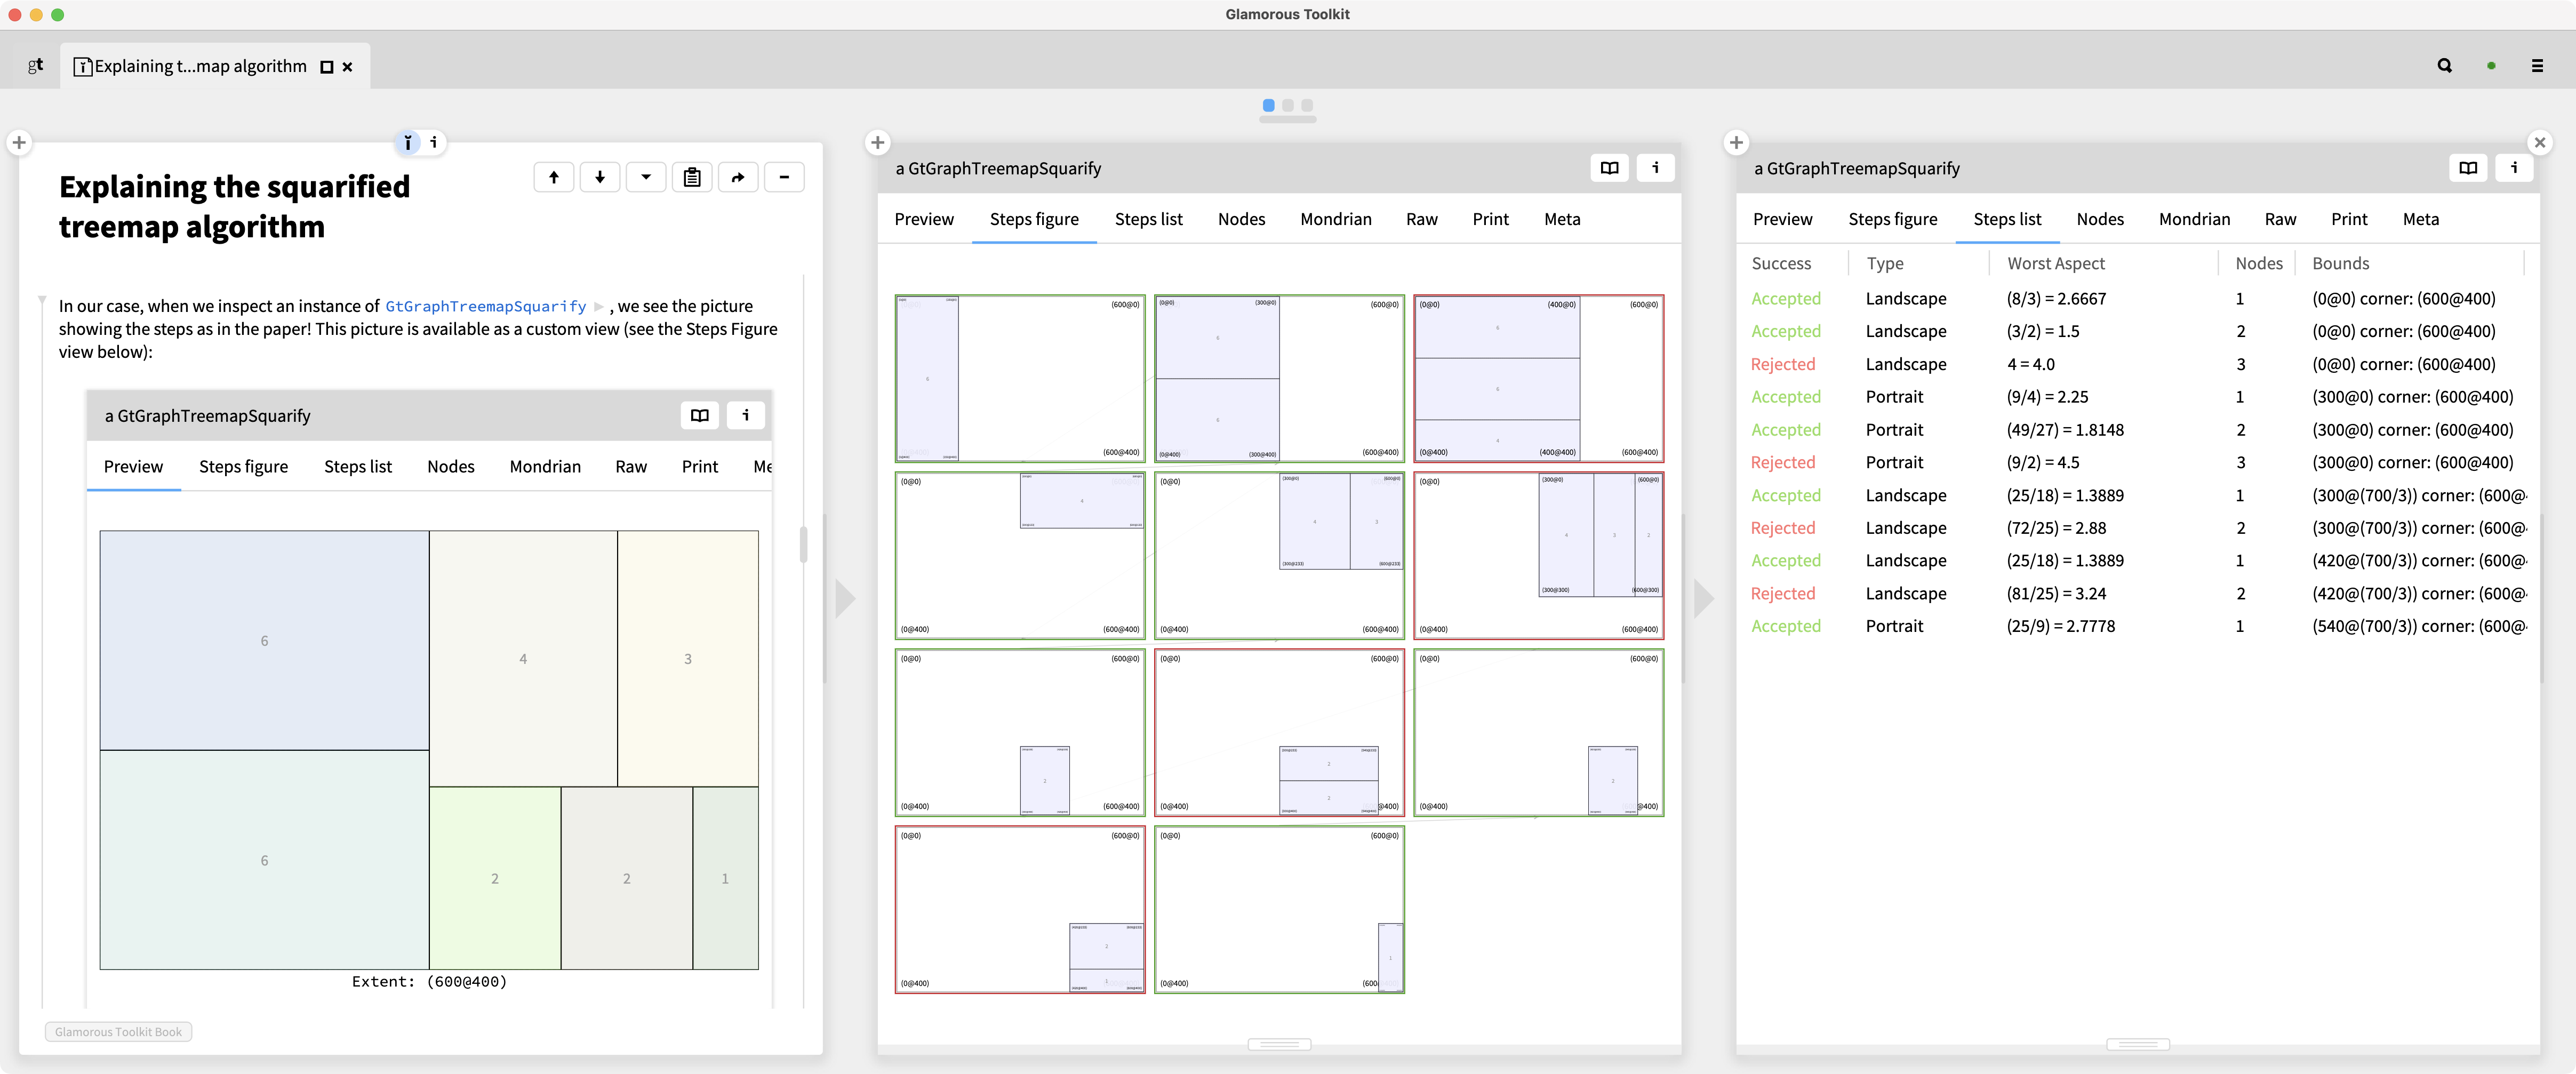
\includegraphics[width=\columnwidth]{book3-Treemap}
  \caption{xxx.}
  \label{fig:Treemap}
\end{figure}




\autoref{fig:Patterns} shows how examples can be used within notebook pages that explain the moldable development process in terms of a number of patterns.
\todo{cite the patterns paper}
\todo{explain the figure}


\begin{figure}[h]
  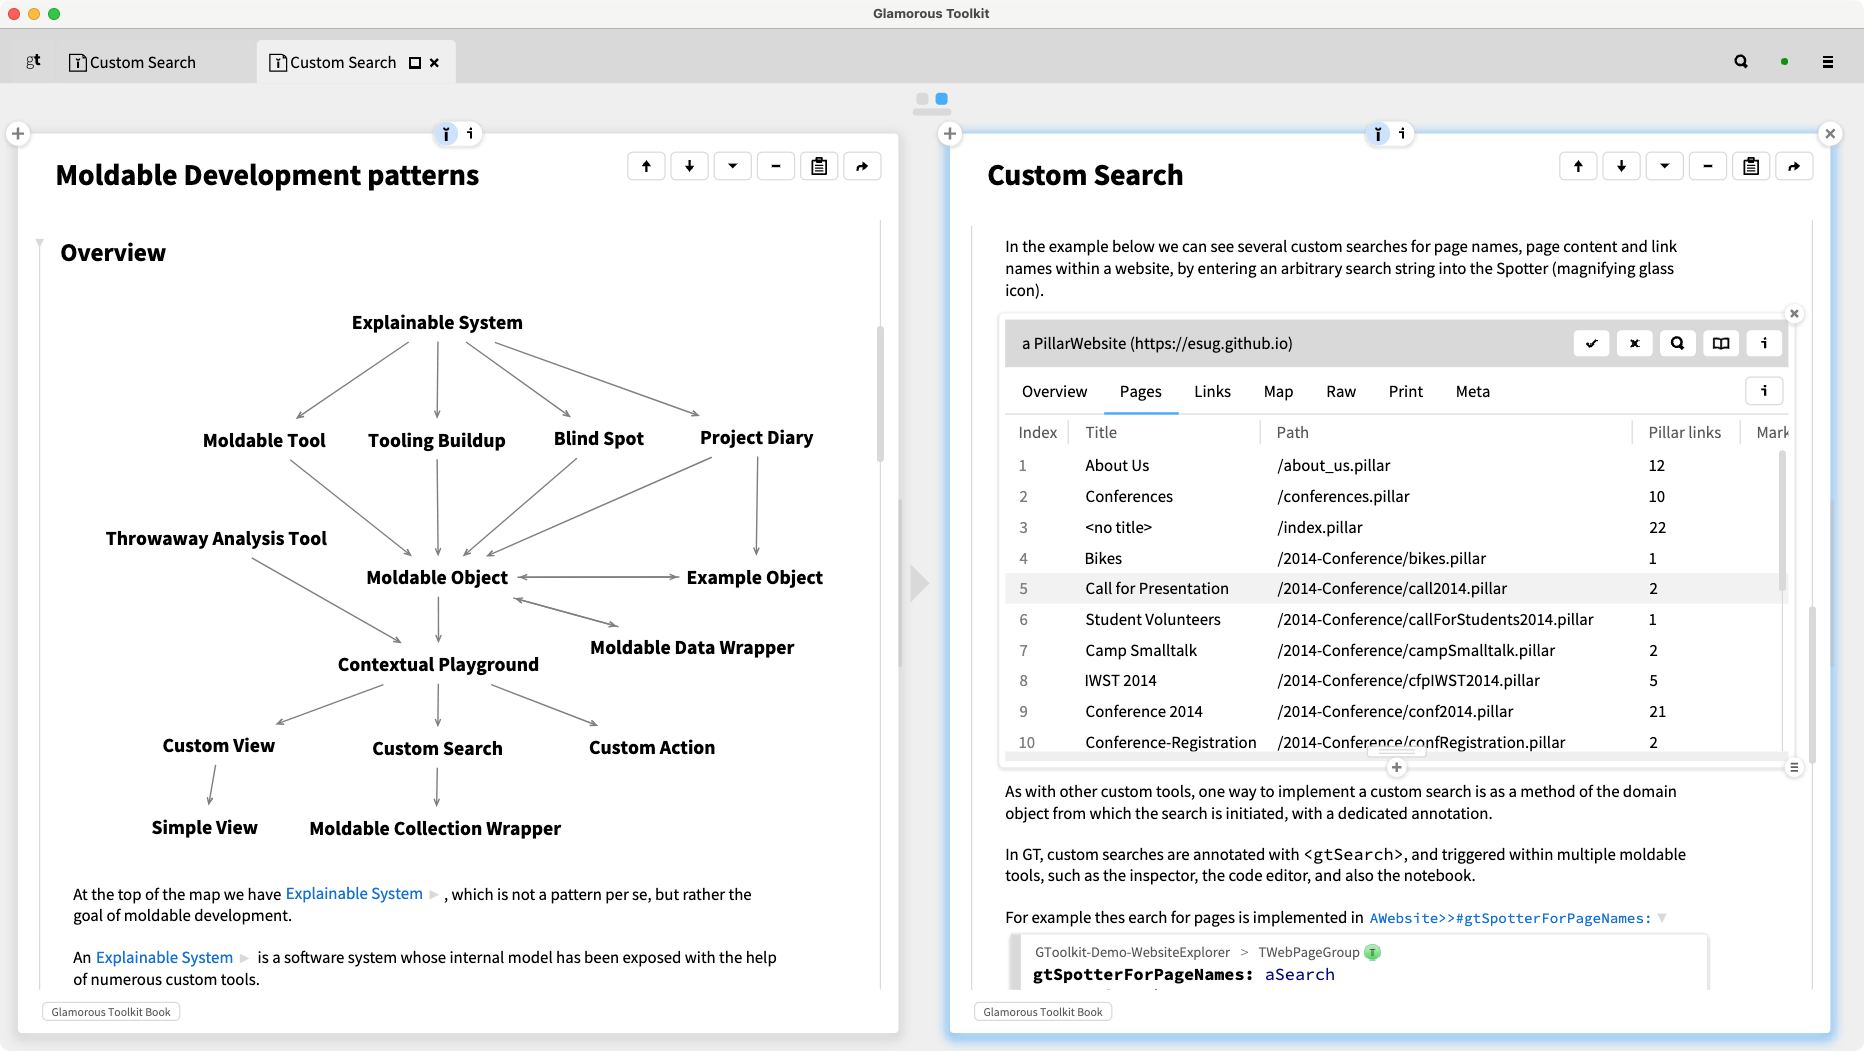
\includegraphics[width=\columnwidth]{book4-MDPatterns}
  \caption{xxx.}
  \label{fig:Patterns}
\end{figure}




All of these illustrations show not only how example methods can be used productively to produce live documentation, but that by applying moldable development principles, the live examples can be easily enhanced with lightweight, custom tools that serve to make the examples, and the systems they are part of, truly explainable.

\todo{statistics on examples, snippets, pages etc.}


% ============================================================
\section{Related work}\label{sec:related}

\todo{Add something on Shri's Examplar paper}
% https://cs.brown.edu/~sk/Publications/Papers/Published/wk-examplar/

The \emph{Test Data Builder} pattern~\cite{Free09a} introduces factory methods for test fixtures, also potentially reducing code duplication in tests, but the resulting objects are only intended as inputs for tests, not their outputs.
The resulting examples are not accessible as the output of a green test.

Cucumber~\cite{Hell17a} is a software tool that supports Behavior-Driven Development through business rules specified in the Gherkin language.
These rules include the specification of ``examples'' (AKA scenarios) that illustrate business rules.
The usage of these examples, however, is restricted to the context of the business rules, and they are not intended as the outputs of tests.

Modern testing frameworks such as pytest~\cite{Okke22a}, allow tests to be parameterized by fixtures specified as separate methods.
Here too, however, fixtures are only seen as inputs to tests, not as outputs.

\todo{Something about notebooks and live examples ...
The idea of notebooks with embedded examples is not new, but combining them with tests and lightweight, custom tools to create narratives is new.}

Bush was the first to dream of a computerized ``memex'' of stored knowledge~\cite{Bush45a}, through which a user could trace an associate ``trail'' of interconnected text and multimedia resources.
The memex inspired Engelbart's NLS~\cite{Enge68a}, the first system to demonstrate human interaction with a computer mouse, windows, and hypertext features.
Knuth first pioneered the implementation of a computational notebook, called WEB, to support ``literate programming'' through the combination of text, graphics, and live code~\cite{Knut97a}.

Modern notebook systems such as Jupyter\footnote{\url{https://jupyter.org}}, MATLAB Live Scripts\footnote{\url{https://www.mathworks.com/}} and Wolfram Notebooks\footnote{\url{https://www.wolfram.com/notebooks/}} all offer the ability to embed live instances of classes within notebook pages, but these live examples are neither integrated with unit testing frameworks, not do they support custom tooling with the help of moldable tools to tailor the user experience.

% ============================================================
\section{Conclusion}\label{sec:conclusion}

\todo{Somewhere refer to MD patterns \cite{Nier24a} and moldable exceptions \cite{Chis24a}?}

\todo{
Summary:\\
- having tests be factories for examples is a tiny, but groundbreaking enhancement\\
- EDD enhances TDD by making examples rather than tests the focus in the development process\\
- by enhancing examples with lightweight, custom tools, they help users answer all kinds of analysis questions\\
- by embedding examples in live documentation, they make software systems explainable.
}

\todo{
Concluding points:\\
- ...
}


%\begin{acks}
%\end{acks}

% ============================================================

\bibliographystyle{ACM-Reference-Format}
\bibliography{eddBridge}

\end{document}
\endinput

% ============================================================

\begin{inparaenum}[(i)]
	\item 
\end{inparaenum}


\begin{figure}[h]
  \includegraphics[width=\columnwidth]{xxx}
  \caption{xxx.}
  \label{fig:xxx}
\end{figure}


